\documentclass[10pt]{article}
\usepackage{fullpage}
\newif\ifacmstyle
\acmstylefalse
\usepackage{lmodern} % More complete than the default CM font
\usepackage[T1]{fontenc} % needed for lmodern
\usepackage[utf8]{inputenc}
%\usepackage{newtxtext} % use (similar to) Times font in text.
%\usepackage{newtxmath} % use (similar to) Times font in math.
\usepackage{hyperref} % Must be loaded before cleveref
\usepackage{cleveref} % to have smart references using \cref.
\crefname{section}{§}{§§}
\Crefname{section}{§}{§§}
\crefformat{section}{§#2#1#3}
\crefname{theorem}{thm.}{thms.}
\Crefname{theorem}{Thm.}{Thms.}
\crefformat{theorem}{Thm.~#2#1#3}
\usepackage{mdwlist} % compressed itemize, enumerate
\usepackage[numbers,sort&compress,square]{natbib}
\renewcommand{\refname}{REFERENCES}
\renewcommand{\bibsection}{\section{REFERENCES}}
\usepackage[ruled,linesnumbered]{algorithm2e} % must be loaded after natbib
\usepackage{amssymb}
\usepackage{graphicx}
\usepackage{url}
\usepackage{color}
\usepackage{soul}
\usepackage{mathtools}
\newcommand*{\defeq}{\coloneqq}
\usepackage{caption}
\usepackage{subcaption}
\usepackage{nicefrac}
\usepackage{floatrow}

\ifacmstyle
\else
\usepackage{amsthm}
\fi
\newtheorem{corollary}{Corollary}
\newtheorem{lemma}{Lemma}
\newtheorem{theorem}{Theorem}
\newtheorem{fact}{Fact}
\newtheorem{conjecture}{Conjecture}
\newtheorem{proposition}{Proposition}
\newtheorem{remark}{Remark}
\ifacmstyle
\else
\theoremstyle{definition}
\fi
\newtheorem{definition}{Definition}

\DeclareMathOperator*{\argmax}{arg\,max}
\DeclareMathOperator*{\argmin}{arg\,min}

\newcommand{\paran}[1]{\left(#1\right)}
\newcommand{\set}[1]{\left\{#1\right\}}
\newcommand{\setof}[2]{\left\{#1 \vert #2\right\}}
% \newcommand{\E}[1]{\mathbb{E}\left(#1\right)}

\newcommand{\pr}[1]{\text{Pr}\left[#1\right]}
\newcommand{\cost}[1]{\text{cost}\left( #1 \right)}
\def\pr{\text{Pr}}
\def\E{\mathbb{E}}
\def\M{{\cal M}}
\def\p{\mathbf{p}}
\def\S{\mathcal{I}}
\def\F{\mathcal{F}}
% \def\I{\mathcal{I}}
\def\T{\mathcal{T}}
\def\P{\mathcal{P}}

    
\def\D{\mathcal{D}}
\def\deg{\text{deg}}
\def\optimizer{\texttt{optimizer}}
\def\appoptimizer{\texttt{approx\_optimizer}}
\def\sampler{\texttt{sampler}}
\def\sys{\Gamma}
\def\fr{\text{fr}}
\def\ins{informed-set}
\def\escos{\text{cost}}
\def\mi{\text{mi}}
\def\probname{Probabilistic Hitting Set Paradigm}
\def\problem{Probabilistic Hitting Set Problem}

\usepackage[show]{notes-alt}


\begin{document}
\title{Fast Approximation of Betweenness Centrality through Sampling}
\author{Ahmad Mahmoody\footnote{Contact author}, Matteo Riondato, Eli Upfal\\
Department of Computer Science -- Brown University \\
\url{{ahmad, matteo, eli}@cs.brown.edu}}

\title{\algonamebasecap: Detecting Valuable Information\\in Dynamic Networks Using Limited Resources}
\maketitle

\textit{``Have you found it, Wiggins?''}
\begin{flushright}
	[Sherlock Holmes in \emph{A Study in Scarlet}]
\end{flushright}

\begin{abstract}
	%\todo[Matteo]{Shorten to fit in single column, with Categories and
	%Keywords.}
	Detecting information spreading across a network can be done by monitoring
	its nodes and has many practical applications: discovering new webpages,
	analyzing influence properties in network, and detecting failure propagation
	in electronic circuits or infections in public drinkable water systems. In
	practice, it is infeasible for anyone but the owner of the network (if
	existent) and government agencies to monitor all nodes at all times. In this
	work we study the constrained setting when the observer can only probe a
	small set of nodes at each time step to check whether new pieces of
	information (items) have reached those nodes.

	We formally define the problem through an infinite time generating process
	that places new items in subsets of nodes according to an unknown
	probability distribution. Items have an exponentially decaying
	\ahmad{\emph{novelty}}, modeling their decreasing value. The observer uses a
	\emph{probing schedule} (i.e., a probability distribution over the set of
	nodes) to choose, at each time step, a small set of nodes to check for new
	items. The goal is to compute a schedule that minimizes the average
	\ahmad{novelty} of undetected items. We present an algorithm, \algoname, to
	compute the optimal schedule through convex optimization, and then show how
	it can be adapted when the parameters of the problem must be learned or
	change over time. We also present a scalable variant of \algoname for the
	MapReduce framework. The results of our experimental evaluation on real
	social networks demonstrate the practicality of our approach.
\end{abstract}


\section{Introduction}\label{sec:introduction}
Many applications require the detection of events in a network as soon as they
happen or shortly thereafter, as the value of the information obtained by
detecting the events decays rapidly as times passes. For example, an emerging
trend in algorithmic stock trading is the use of automatic search through the
Web and social networks for pieces of information that can be used in trading
decisions before they appear in the more popular news
sites~\citep{Delaney2009,ALPHA2014,AlphaFlash,mitra2011handbook,latar2015robot,wallstreet2015,McKinney2011}.
\mynote[All]{Do we really want all these newspaper journals and software
	manuals in the references? I would love to cite the TwoSigma
	one~\citep{wallstreet2015}, obviously ;), but it seems a bit too much to
have 7 references for this?}
Similarly, intelligence, business and politics analysts are scanning online
sources for new information or rumors. While new items are often reblogged,
retweeted, and posted on a number of sites, it is sufficient to find an item
once, as fast as possible, before it loses its relevance. There is no benefit in
seeing more copies of the same news item, or rumor. A similar situation also
arises in the need to detecting intrusions, infections, or defects in,
respectively, a computer network, a public water system, or a large electronic
circuit.

Indeed this is a fundamental search and detection problem in a distributed data
setting, not limited to social networks or graph analysis. In this setting, the
data is distributed among a large number of nodes, and new items appear in
individual nodes (for example, as the products of processing the data available
locally at the node), and may propagate (being copied) to neighboring nodes on a
physical or a virtual network. The goal is to detect at least one copy of each
new item as soon as possible. The search application can access any node
in the system, but it can only \emph{probe} (i.e., check for new items on) a few
nodes at a time. To minimize the time to find new items, the search application
needs to optimize the schedule of probing nodes, taking into account (i) the
distribution of copies of items among the nodes (to see where to probe), and
(ii) the decay of items' \emph{\ahmad{novelty}} (or relevance) over time (to focus the
search on most relevant items). The  main challenge is in devising a good
probing schedule in absence of prior knowledge on the generation and
distribution of items in the network.

% Commented by Matteo on 06/29
%Another application that faces a similar search problem is processing security
%raw data (e.g. gathered security raw footages that need to be processed).
%Ideally, given limited resources compared to the huge volume of the data, a
%schedule for processing (probing) different raw-dataset has to minimize the
%value of missing information (assuming newer information are more valuable than
%older ones).

\paragraph*{Contributions}
In this work we study the problem of computing an optimal node probing schedule
for detecting new items in a network under resource scarceness, i.e., when only
a few nodes can be probed at a time. Our contributions to the study of this
problem are the following:

\begin{itemize*}
	\item We formalize a generic process that describe the creation and
		distribution of information in a network and clearly define the task of
		studying this process by probing the nodes in the network according to a
		schedule. The process and task are parametrized by the resource
		limitations of the observer and the decay rate of the \ahmad{novelty} of
		items. We then introduce a \emph{cost} measure to compare different
		schedules. The cost of a schedule is the limit of the average expected
		\ahmad{novelty} of uncaught items at each time step.
		\todo[Matteo]{Mention the actual name of the problem we study.}
	\item We conduct a theoretical study of the cost of a schedule, showing that
		it can be computed explicitly and that is a convex function over the
		space of schedules. We then introduce \algoname,\footnote{In the Sherlock
			Holmes novel \emph{A study in scarlet} by A.~Conan Doyle, Wiggins is
			the leader of the ``Baker Street Irregulars'', a band of street
			urchins employed by Holmes as intelligence agents.} an algorithm to
		compute the optimal schedule by solving a constrained convex
		optimization problem.
		\todo[Matteo]{Mention iterative method through Lagrange multipliers.}
	\item We discuss variants of \algoname for the realistic situation where
		the parameters of the process needs to be learned or can change over
		time. Among these variants, we present an adaptation for the MapReduce
		framework of computation, which allow us to handle very large networks.
		\todo[Matteo]{Mention approx quality.}
	\item Finally, we conduct an extensive experimental evaluation of \algoname
		and its variants, comparing the performances of the schedules it
		computes with natural baselines, and showing how it performs extremely
		well in practice on real social networks when using well-established
		models for generating new items (e.g., the independence cascade
		model~\citemissing).
\end{itemize*}

To the best of our knowledge, the problem we study is novel and we are the first
to devise an algorithm to compute an optimal schedule, both when the generating
process parameters are known and when they need to be learned. Many variants
of the problem we introduce can be devised but, due to lack of space, we defer
their study to the extended version of this work.

\para{Paper Organization} In Sect.~\ref{sec:prelims} we give introductory
definitions and formally introduce the settings and the problem. We discuss
related works in Sect.~\ref{sec:related_work}. In Sect.~\ref{sec:method} we
describe our algorithm \algoname and its variants. The results of our
experimental evaluation are presented in Sect.~\ref{sec:exp}. We conclude by
outlining directions for future work in Sect.~\ref{sec:concl}.

\section{Problem Definition}\label{sec:prelims}
In this section we formally introduce the problem and define our goal.

Let $G=(V,E)$ be a graph with $|V|=n$ vertices. W.l.o.g.~we let $V=[n]$. Let
$\family\subseteq 2^V$ be a collection of subsets of $V$, i.e., a collection of
sets of nodes. Let $\pi$ be a function from $\family$ to $[0,1]$ (not
necessarily a probability distribution). We model the generation and diffusion
of information information in the network by defining a \emph{generating
process} $\sys=(\family,\pi)$.  $\sys$ is a infinite discrete-time process
which, at each time step $t$, generates a set $\Sample_t\subseteq\family$ such
that $S\in\family$ is included in $\Sample_t$ with probability $\pi(S)$,
independently of $t$ and of other sets generated at time $t$ and at time $t'<t$.
For any $t$ and any $S\in\Sample_t$, we call the ordered pair $(t,S)$ an
\emph{item}, representing a piece of information that was generated at time $t$
and reached \emph{instantaneously} the nodes in $S$.  We choose to model the
diffusion process as instantaneous because it appears as such to a
resource-limited observer who does not have the resources to monitor all the
network at the fine time granularity needed to observe the different stages of
the diffusion process.

\para{Probing and schedule} The observer can only monitor the network by
\emph{probing} nodes. Formally, by \emph{probing a node $v\in V$ at time $t$},
we mean obtaining the set $I(t,v)$ of items $(t',S)$ such
that $t'\le t$ and $v\in S$:
\[
	I(t,v)\defeq\{(t',S) ~:~ t'\le t, S\in\Sample_{t'}, v\in S\}\enspace.
\]
Let $U_t$ be the union of the sets $\Sample_{t'}$ generated by $\sys$
at any time $t'\le t$, then we have $I(t,v)\subseteq U_t$. We assume that
probing a node is not a computationally expensive operation: probing a node $v$
at time $t$ gives immediate access to $I(t,v)$. This is a realistic assumption:
for example, accessing the profile of a user in a social network gives access to
the list of items that reached that user.

We model the \emph{resource limitedness of the observer} through a constant,
user-specified, parameter $c\in\mathbb{N}$, representing the maximum number of
nodes that can be probed at any time $t$.

The observer chooses the $c$ nodes to probe by following a schedule. In this work
we focus on \emph{memoryless} schedules, i.e., the choice of nodes to probe at
time $t$ is independent from the choice of nodes to probe at any time $t'<t$.
More precisely, a \emph{probing $c$-schedule} $\sched$ is a probability
distribution on $V$. At each time $t$, the observer chooses as set $P_t$ of $c$
nodes to probe, such that $P_t$ is obtained through \emph{random sampling of $V$
without replacement according to $\sched$}, independently from $P_{t'}$ from
$t'< t$. We postpone the study of adaptive or sequential schedules to future
work.

\para{Caught items, uncaught items, and freshness}
We say that an item $(t',S)$ is \emph{caught at time $t\ge t'$} iff
\begin{enumerate*}
	\item a node $v\in S$ is probed at time $t$; and
	\item no node in $S$ was probed in the interval $[t',t-1]$.
\end{enumerate*}

Let $C_t$ be the set of items caught by the observer at any time $t'\le t$. We
have $C_t\subseteq U_t$. Let $N_t= U_t\setminus C_t$ be the \emph{set of
uncaught items at time $t$}, i.e., items that were generated at any time
$t'\le t$ and have not been caught yet at time $t$. For any item $(t',S)\in
N_t$, we define the \emph{$\theta$-freshness of $(t',S)$ at time $t$} as
\[
	\fresh_\theta(t,t',S)\defeq\theta^{t-t'},
\]
where $\theta\in(0,1)$ is a user-specified parameter modeling how fast the
value of an item decreases with time if uncaught. Intuitively, pieces of
information (e.g., rumors) have high value if caught almost as soon as they have
appeared in the network, but their value decreases fast (e.g., exponentially) as
more time passes before being uncaught, to the point of having no value in the
limit. In the rest of the paper we drop the $\theta$ from the notation of
freshness of an item at time $t'$ as it will be clear from the context.

\para{Load of the system and cost of a schedule} The set $N_t$ of uncaught items
at time $t$ imposes a \emph{$\theta$-load $L_\theta(t)$ on the graph at time
$t$}, defined as the sum of the $\theta$-freshness at time $t$ of the items in
$N_t$:
\[
	L_\theta(t)\defeq\sum_{(t',S)\in N_t} \fresh_\theta(t,t',S)\enspace.
\]
The quantity $L_\theta(t)$ is a random variable, depending both on $\sys$ and on
the probing schedule $\sched$, and as such it has an expectation
$\expect[L_\theta(t)]$ w.r.t.~all the randomness in the system. The
\emph{$\theta$-cost of a schedule $\sched$} is defined as the limit, for
$t\rightarrow\infty$, of the average expected load of the system:
\[
	\cost_\theta(\sched)\defeq\lim_{t\rightarrow\infty}\frac{1}{t}\sum_{t'\le
	t}\expect[L_\theta(t)]=\lim_{t\rightarrow\infty}\frac{1}{t}\sum_{t'\le
	t}\expect\left[\sum_{(t'',S)\in N_{t'}}\fresh_\theta(t',t'',S)\right]\enspace.
\]
\todo{Add some motivation/intuition for this choice of cost measure.}
The limit above always exists as proven in Lemma~\ref{lem:explicit}.
\todo{Is the proof of existence actually there?}

We now have all the necessary ingredients to formally define the problem of
interest in this work.

\para{Problem definition} Let $G=(V,E)$ be a graph and $\sys=(\family,\pi)$ be a
generating process on $G$. Let $c\in\mathbb{N}$ and
$\theta\in(0,1)$. The \emph{$(\theta,c)$-Optimal Probing Schedule Problem}
($(\theta,c)$-OPSP) requires to find the \emph{optimal $c$-schedule} $\sched^*$,
i.e., the schedule with \emph{minimum} $\theta$-cost over the set $\mathsf{S}_c$
of $c$-schedules.
\[
	\sched^*=\argmin\{\cost_\theta(\sched), \sched\in\mathsf{S}_c\}\enspace.
\]

In other words, the goal is to design a $c$-schedule that allows to catch items
that have higher freshness (which correspond to those generated most recently).
Tthe parameter $\theta$ controls how fast the freshness of an item decays, i.e.,
how fast they loose value for the agent. A value of $\theta$ very close to $0$
requires to catch the item  as soon as they are generated (or at most shortly
thereafter). At the other extreme ($\theta\approx 1$), an ideal schedule should
try to maximize the number of caught items, as their freshness decays very
slowly. In other words, the optimal schedule is such that elements of $U$ more
likely to receive ``fresh'' items have higher probability of being probed.
Intuitively, if we see the items as the ``information'' flowing in the network,
then an ideal schedule should assign higher probability of being probed to nodes
that act as \emph{fresh information hubs}, i.e., receive a large number of
items. Hence by examining the optimal schedule $\sched$, we can identify
information hubs among the nodes. This task (finding information hubs) can be
seen as the complement of the \emph{influence maximization
problem}~\citep{Kempe2003,Kempe2005}. In the influence maximization problem we
look for a set of nodes that \emph{generate} information that reach most nodes.
In the information hubs problem we are interested in a set of nodes that
\emph{receive} the most of information, thus the most informative nodes for an
observer.

In the following sections, we almost often drop the specification of the
parameters from $\theta$-freshness, $\theta$-cost, $\theta$-load, and
$c$-schedule, and from their respective notation, as the parameters will be
clear from the context.

% Commented by Matteo on 6/30
%In a social network, news and pictures are shared and re-shared over time, and
%each such shared ``item'' reaches a certain set of users. A resource-limited
%agent is interested in knowing what items get shared on the network. Also, the
%agent would like to know as soon as possible that an item has been shared,
%because the value of this piece of information decreases over time. Being
%resource-limited, the only way that the agent can observe (catch) the sharing of
%items is to probe some nodes (i.e., users) of the social network, for example by
%accessing their profile and getting a list of the items that they received from
%other users or that they shared. Therefore, the agent needs a probing schedule
%that allows her to catch as many items as possible while minimizing the time
%between the sharing of an item and its being caught. Equivalently, the schedule
%must be such that the ``value'' of the information that is not caught by the
%agent is minimized. Intuitively, the schedule must be such that nodes that
%receive a high number of items shortly after they have been generated should
%have a higher probability of being probed. These nodes act, in some sense, as
%``information hubs''. As such, identifying them can be seen as the complement of
%the \emph{influence maximization problem}~\citep{Kempe2003,Kempe2005}. In the
%influence maximization problem we look for a set of nodes that \emph{generate}
%information that reach most nodes. In the information hubs problem we are
%interested in a set of nodes that \emph{receive} the most of information, thus
%the most informative nodes for an observer.

\section{Related Work}\label{sec:related_work}
The novel problem we focus on in this work generalizes and complements a number of problems
studied in the literature.

The  ``Battle of Water Sensor Network'' challenge~\citep{BWSN2008} motivated a
number of works on \emph{outbreak detection}: the goal is to optimally place
static or moving sensors in water networks to detect
contamination~\citep{Leskovec2007,Krause2008,Hart2010}. The optimization can be
done w.r.t.~a number of objectives, such as maximizing the probability of
detection, minimizing the detection time, or minimizing the size of the
subnetwork affected by the phenomena~\citep{Leskovec2007}. A related
work~\citep{AgumbeSuresh2012} considered sensors that are sent along fixed paths
in the network with the goal of gathering sufficient information to locate
possible contaminations. Early detection of contagious outbreaks by monitoring
the neighborhood (friends) of a randomly chosen node (individual) was studied
by~\citet{Christakis2010}.  \citet{Krause2009} present efficient schedules for
minimizing energy consumption in battery operated sensors, while other works
analyzed distributed solutions with limited communication capacities and
costs~\citep{Krause2011Kleinberg,Golovin2010,Krause2011}. % spacesaver
%Another objective in the Sensor Placement problem is to {\bf predict} the phenomena at locations without sensors (e.g., road speeds on highways).  studies this problem where there is restriction on the battery life of the sensors, and thus, the sensors need to be placed and \emph{scheduled} such that at each time just some of the sensors are \emph{active}. Also, \cite{Golovin2010} studies the same problem and provides a distributed solution where the sensors are not connected to a centralized optimizer and they activate themselves using local information. \cite{Krause2011} presents an algorithm in which sensors have to communicate through
%lossy channels in environmental monitoring, and \cite{Krause2011Kleinberg} brings the communication cost into account.
In contrast, our work is geared to detection in huge but virtual networks such
as the Web or social networks embedded in the Internet, where it is possible to
``sense'' or probe (almost) any node at approximately the same cost. Still only
a restricted number of nodes can be probed at each steps but the optimization of
the probing sequence is over a much larger domain, and the goal is to identify
the outbreaks (items) regardless of their size and solely by considering their
interest value.

%An interesting related research direction aims at \emph{controlling} or
%\emph{stopping} contagions in the networks by changing the topology of the
%network (e.g, by protecting or blocking the edges and/or
%nodes)~\cite{Aspnes2006,Kimura2008Minimizing,Kimura2008,Kimura2009,Li2011,He2011,Kuhlman2013}. %
%In our model, though, probing the nodes is the only action we can take.}
%%%%%%%%%%%%%%
%\emph{Anomaly Detection} instead requires to find the events (usually
%structural) that deviate from \emph{normal}
%patterns~\cite{Noble2003,Sun2007,Eberle2007,Papadimitriou2010,Akoglu2010,Bogdanov2013}.
%%%%%%%%%%%%%%%%

Our methods complement the work on \emph{Emerging Topic Detection} where the
goal is to identify emerging topics in a social network, assuming full access to
the stream of all postings. Providers, such as Twitter or Facebook, have an
immediate access to all tweets or postings as they are submitted to their
servers~\cite{Cataldi2010,Mathioudakis2010}. Outside observers need an efficient
mechanism to monitor changes, such as the methods developed in this work.

\emph{Web-crawling} is another research area that study how to obtain the
most recent snapshots of the web. However, it differs from our model in two key
points: our model allows items to propagate their copies, and they will be
caught if any of their copies is discovered (where snapshots of a webpage belong
to that page only), and all the generated items should be discovered (not
just the recent ones)~\cite{dasgupta2007discoverability,wolf2002optimal}.

The goal of the {News and Feed Aggregation} problem is to capture updates in news websites (e.g. by RSS feeds)~\cite{survey-oita2011deriving,onlineRef-horincar2014online,adaptive-bright2006adaptive,fast-sia2007efficient}. Our model differs from that setting in that we consider copies of the same news in different web sites as equivalent and therefore are only interested in discovering one of the copies.


%\ahmad{
%The \emph{News and Feed Aggregation} problem is a very well-studied topic, in which the general goal is to obtain the updates of news websites (e.g. by RSS feeds). Among many introduced objectives~\cite{survey-oita2011deriving,onlineRef-horincar2014online,adaptive-bright2006adaptive} in studying this problem, the most similar one to our cost function is the \emph{delay} function presented by~\cite{fast-sia2007efficient}.  In~\cite{fast-sia2007efficient} it is assumed that the rates of the news publication does not change, where in our setting these rates may change and our algorithm ({\ada}) can adapt itself to the new setting. Also, we assume at any given time the number of probes is fixed (or bounded) regarding the limited computational power for simultaneous probes, but \cite{fast-sia2007efficient} uses a relaxed  assumption by fixing the number of probes over a \emph{time window} of a fixed length which may result in high number of probes at a single time step. Finally, \cite{fast-sia2007efficient} introduces a deterministic algorithm in which the number of probes to each feed is obtained by applying the Lagrange multipliers method (very similar result to Theorem~\ref{thm:randomized_schedule}), but they loose the guarantee on optimality of their solution, by rounding the estimated number of probes to integers. In contrast, our solution provides  theoretical guarantee on optimality of our output schedule. }


% Finally, there are many work on Influence Maximization  and the social network Centrality, but as explained in previous section, they are ``orthogonal'' to  1-PHSP. To see the work on Influence Maximization and Betweenness centrality you can refer to \cite{Kempe2007,Borgs} and \cite{Yoshida}, and their related work.

% Finally, the well-studied problem of \emph{Influence Maximization} problem aimed at optimizing the location of nodes to seed new items, in order to obtain maximum spread of the items~\cite{Kempe2003,Kempe2005,Kempe2007,Chen2009,Chen2010,Goyal2011,Seeman13}.




% % % % % % % % % % % % % % % % % % % % % % % % %
% % % % % % Section: Related   work % % % % % % %
% % % % % % % % % % % % % % % % % % % % % % % % %
% \section{Related work}\label{sec:related_work}
% There has been an extensive work on \emph{outbreak detecdion} in physical domains, in particular the "Battle of Water Sensor Network" challenge~\cite{BWSN2008}  for optimal placement of static sensors in water networks to detect contamination~\cite{Leskovec2007,Krause2008,Hart2010}.
% The optimization is done with respect to different objectives, such as maximizing the probability of detection, minimizing the detection time, or minimizing the size of the subnetwork affected by the phenomena~\cite{Leskovec2007}. A related work~\cite{AgumbeSuresh2012} considered  sensors that are sent along fixed paths in the network with the goal of gathering sufficient information to locate possible contaminations. Early detection of contagious outbreaks
% by monitoring the neighborhood (friends) of a randomly chosen node (individual) was studied in~\cite{Christakis2010}. Efficient scheduling for minimizing energy consumption in battery operated sensors were studied in~\cite{Krause2009}, and distributed solutions with limited communication capacities and costs were studied in~\cite{Krause2011Kleinberg, Golovin2010, Krause2011}.
%
% %Another objective in the Sensor Placement problem is to {\bf predict} the phenomena at locations without sensors (e.g., road speeds on highways).  studies this problem where there is restriction on the battery life of the sensors, and thus, the sensors need to be placed and \emph{scheduled} such that at each time just some of the sensors are \emph{active}. Also, \cite{Golovin2010} studies the same problem and provides a distributed solution where the sensors are not connected to a centralized optimizer and they activate themselves using local information. \cite{Krause2011} presents an algorithm in which sensors have to communicate through
% %lossy channels in environmental monitoring, and \cite{Krause2011Kleinberg} brings the communication cost into account.
% %
% In contrast to these works our work is geared to detection in virtual networks such as the Web or social networks embedded in the Internet, where a monitor can reach (almost) any node at about the same cost. The monitor is still restricted to probing a small number of nodes per step, but the optimization of the probing sequence is over a larger and more complex domain.
%
% \ahmad{Another trend of studies, aim to \emph{controlling} or \emph{stopping} contagions in the networks by changing the topology of the network (e.g, by protecting or blocking the edges and/or nodes)~\cite{Aspnes2006,Kimura2008Minimizing,Kimura2008,Kimura2009,Li2011,He2011,Kuhlman2013}. In our model, though, probing the nodes is the only action we can take.}
%
% Our methods complement the work on \emph{Emerging Topic Detection} where the goal is to identify emergent topics in a social network, assuming full access to the stream all posting. Providers, such as Twitter of Facebook, have an immediate access to all tweets or postings as they are submitted to their server~\cite{Cataldi2010,Mathioudakis2010}. Outside observers need an efficient mechanism to monitor changes.
%
% %%%%%%%%%%%%%%
% \ahmad{
% There is a rich work in the area of \emph{Anomaly Detection} whose goal is to find the events (usually structural) that deviate from a \emph{normal} pattern, e.g see \cite{Noble2003,Sun2007,Eberle2007,Papadimitriou2010,Akoglu2010,Bogdanov2013}. In our work we assume a fixed set of parameters, and rather focusing on the pattern of the events (e.g., pattern of the subnetwork that an item has reached) we are interested in catching (all) the items.
% }
% %%%%%%%%%%%%%%%%
%
% Finally, the well-studied problem of \emph{Influence Maximization} problem aimed at optimizing the location of nodes that generated new items to obtain maximum spread of the items~\cite{Kempe2003,Kempe2005,Kempe2007,Chen2009,Chen2010,Goyal2011,Seeman13}. \ahmad{Note that the goal in Influence Maximization problem is to spread the items to the largest \emph{size}, while reversely, we aim to detect the items in shortest \emph{time}.}
%
% % \ahmad{ \st{measuring the influence of people }~\cite{Weng2010,Cha2010}}
%
%
%

\section{The \algonamebasecaps{} Algorithm}\label{sec:method}
In this section, we study the $(\theta,c)$-OPSP for a generating process
$\sys=(\family,\pi)$ on a graph $G=(V,E)$ and present the algorithm \algoname
(and its variants) to solve it.

We start we start by assuming that we have complete knowledge of $\sys$, i.e.,
we know $\family$ and $\pi$. This strong assumption allows us to study the
theoretical properties of the cost of a function and motivates the design of
our algorithm \algoname to compute an optimal schedule. We then remove the
assumption and show how we can extend \algoname to only use a collection of
observations from $\sys$. Then we discuss how to recalibrate our algorithms when
the parameters of the process (e.g., $\pi$ or $\family$) change over time.
Finally, we show an algorithm for the MapReduce framework that allows us to
scale to large networks.

\subsection{Computing the Optimal Schedule}\label{sec:optimize}
We now first conduct a theoretical analysis of the cost function $\cost_\theta$,
and then use the results to develop \algoname, our algorithm to compute the
optimal $c$-schedule (i.e., solve the $(\theta,c)$-OPSP).

\paragraph{Analysis of the cost function}
Assume for now that we know $\sys$, i.e., we have complete knowledge $\family$,
and $\pi$. With this assumption, we can exactly compute the $\theta$-cost of a
$c$-schedule.

\begin{lemma}\label{lem:explicit}
Let $\sched$ be a $c$-schedule. Then
\begin{equation}\label{eq:explicit}
	\cost(\sched) \defeq
	\lim_{t\rightarrow\infty}\frac{1}{t}\sum_{t'=0}^t\expect[L_\theta(t')] =
	\sum_{S\in \family} \frac{\pi(S)}{1- \theta(1-\sched(S))^c},
\end{equation}
where $\sched(S) = \sum_{v\in S} \sched_v$.
\end{lemma}

\todo[All]{I reorganized the proof, so please review.}
\begin{proof}
	Let $t$ be a time step, and consider the quantity $\expect[L_\theta(t)]$. By
	definition we have
	\[
		\expect[L_\theta(t)]=\expect\left[\sum_{(t',S)\in
		N_t}\fresh_\theta(t,t',S)\right]=\expect\left[\sum_{(t',S)\in
		N_t}\theta^{t-t'}\right],
	\]
	where $N_t$ is the set of uncaught items at time $t$. Let now, for any
	$t'\le t$, $N_{t,t'}\subseteq N_t$ be the set of uncaught items in the form
	$(t',S)$. Then we can write
	\[
		\expect[L_\theta(t)]=\expect\left[\sum_{t'=0}^{t}\sum_{(t',S)\in
			N_{t,t'}}\theta^{t-t'}\right]\enspace.
	\]
	Define now, for each $S\in\family$, the random variable $X_{S,t',t}$ which
	takes the value $\theta^{t-t'}$ if $(t',S)\in N_{t,t'}$, and $0$ otherwise.
	Using the linearity of expectation, we can write:
	\begin{align}\label{eq:loadexp}
		\expect[L_\theta(t)]&=\sum_{S\in\family}\sum_{t'=0}^t\expect[X_S,t',t]\nonumber\\
		&=\sum_{S\in\family}\sum_{t'=0}^t
		\theta^{t-t'}\Pr(X_{S,t,t'}=\theta^{t-t'})\enspace.
	\end{align}

	The r.v. $X_{S,t,t'}$ takes value $\theta^{t-t'}$ if and only if the
	following two events $E_1$ and $E_2$ both take place:
	\begin{itemize*}
		\item $E_1$: the set $S\in F$ belongs to $\Sample_{t'}$, i.e., is
			generated by $\sys$ at time $t'$;
		\item $E_2$: the item $(t',S)$ is uncaught at time $t$. This is
			equivalent to say that no node $v\in S$ was probed in the time
			interval $[t',t]$.
	\end{itemize*}
	We have $\Pr(E_1)=\pi(S)$, and
	\[
		\Pr(E_2)=(1-\sched(S))^{c(t-t')}\enspace.
	\]
	The events $E_1$ and $E_2$ are independent, as the event of process of
	probing the nodes is independent from the process of generating items,
	therefore, we have
	\[
		\Pr(X_{S,t,t'}=\theta^{t-t'})=\Pr(E_1)\Pr(E_2)=\pi(S)(1-\sched(S))^{c(t-t')}\enspace.
	\]
	We can plug this quantity in the rightmost term of~\eqref{eq:loadexp} and
	write
	\begin{align}
		\expect[L_\theta(t)]&=\sum_{S\in\family}\sum_{t'=0}^t\theta^{t-t'}\pi(S)(1-\sched(S))^{c(t-t')}\nonumber\\
		&=\sum_{S\in\family}\pi(S)\sum_{t'=0}^t(\theta(1-\sched(S))^c)^{t'}\nonumber\\
		&=\sum_{S\in\family}\frac{\pi(S)}{1-\theta(1-\sched(S))^c},
	\end{align}
	where we used the fact that $\theta(1-\sched(S))^c< 1$. Hence the quantity
	$\expect[L_\theta(t)]$ does not depend on $t$, and we have
	\begin{align*}
		\cost_\theta(\sched)&=\lim_{t\rightarrow\infty}\frac{1}{t}\sum_{t'=0}^t\expect[L_\theta(t)]\\
		&=\lim_{t\rightarrow\infty}\frac{1}{t}t\sum_{S\in\family}\frac{\pi(S)}{1-\theta(1-\sched(S))^c}\\
		&=
		\sum_{S\in\family}\frac{\pi(S)}{1-\theta(1-\sched(S))^c}\enspace.
	\end{align*}
\end{proof}

We now show that $\cost_\theta(\sched)$, as expressed by the
r.h.s.~of~\eqref{eq:explicit} is a convex function over its domain
$\mathsf{S}_c$, the set of all possible $c$-schedules. We then use this result
to show how to compute an optimal schedule.

\begin{theorem}\label{thm:convexity}
	The cost function $\cost_\theta(\sched)$ is a convex function over
	$\mathsf{S}_c$.
\end{theorem}
\begin{proof}
	For any $S\in\family$, let
	\[
		f_S(\sched) = \frac{1}{1 - \theta(1-\sched(S))^c}\enspace.
	\]
	The function $\cost_\theta(\sched)$ is a linear combination of
	$f_S(\sched)$'s with positive coefficients. Hence to show that
	$\cost_\theta(\sched)$ is convex it is sufficient to show that, for any
	$S\in\family$, $f_S(\sched)$ is convex.

	We start by showing that $g_S(\sched) = \theta(1-\sched(S))^c$ is convex.
	This is because its Hessian matrix is positive semidefinite. Indeed we have:
	\[
		\frac{\partial}{\partial \sched_i \partial \sched_j} g_S(\sched)=\left\{
		\begin{array}{lr}
		\theta c(c-1) (1-\sched(S))^{c-2} &  i,j \in S\\
		0 &  \text{otherwise}
		\end{array}
		\right.
	\]
	Let $\mathbf{v}_S$ be a $n\times 1$ vector in $\mathbb{R}^n$ such that its
	$i$-th coordinate is $\left[c(c-1) (1-\sched(S))^{c-2} \right]^{1/2}$ if $i\in
	S$, and $0$ otherwise. We can write the Hessian matrix of $g_S$ as
	\[
		\nabla^2 g_S = V_S * V_S^\mathsf{T},
	\]
	and thus, $\nabla^2 g_S$ is positive semidefinite matrix and $g$ is convex.
	From here, we have that $1-g_S$ is a \emph{concave} function. Since
	$f_S(\sched)=\frac{1}{1-g_S(\sched)}$ and the function $h(x)=\frac{1}{x}$ is
	convex and non-increasing, then $f_S$ is a convex function.
\end{proof}

If for every $v\in V$, $S=\{v\}$ belongs to $\family$, then the
function $g_S$ in the above proof is \emph{strictly} convex, and so is $f_S$.

We then have the following corollary of Thm.~\ref{thm:convexity}.

\begin{corollary}\label{corol:convexity}
	Any schedule $\sched$ with locally minimum cost is an optimal schedule
	(i.e., it has global minimum cost). Furthermore, if for every $v\in V$,
	$\{v\}$ belongs to $\family$, the optimal schedule is \emph{unique}.
\end{corollary}

\paragraph{The algorithm}
Corollary~\ref{corol:convexity} implies that one can compute an optimal
$c-$schedule $p^*$ (i.e., solve the $(\theta,c)$-OPSP) by solving the
unconstrained minimization of $\cost_\theta$ over the set $\mathsf{S}_c$ of all
$c$-schedules, or equivalently by solving the following constrained minimization
problem on $\mathbb{R}^+$:
\begin{equation}\label{eq:optimization}
	\boxed{
	\begin{array}{rrclcl}
	\displaystyle \min_{\sched\in\mathbb{R}_n} & \multicolumn{3}{l}{\cost{\sched}} \\
	&\displaystyle \sum_{i=1}^{n} \sched_i & = & 1 \\
	&\sched_i & \geq & 0 & & \forall i \in \{1,\ldots,n\} \\
	\end{array} }
\end{equation}
Since the function $\cost_\theta$ is convex and the constraints are linear, the
optimal solution can, theoretically, be found efficiently~\citep{BoydV04}. In
practice though, available convex optimization problem solvers can not scale
well with the number $n$ of variables, especially when $n$ is in the millions,
as is the case for modern graphs like online social networks or the Web. Hence
we developed \algoname, an iterative method based on \emph{Lagrange
multipliers}\citemissing, which can scale efficiently and can be adapted to the
MapReduce framework of computation~\citep{dean2008mapreduce}, as we show in
Sect.~\ref{sec:mapreduce}.
\todo[Ahmad]{You mentioned something about main memory as motivation for using
	the iterative method, please add that observation here.}
While we can not prove that this iterative method
always converges, we can prove that (i) if at any iteration the algorithm
examines an optimal schedule, then it will reach convergence at the next
iteration, and (ii) if it converges to a schedule, that schedule is optimal (see
Thm.~\ref{thm:optimal}). In Sect.~\ref{sec:exp} we show our experimental results
illustrating the convergence of \algoname in different cases.

\algoname takes as inputs the collection $\family$, the function $\pi$, and the
parameters $c$ and $\theta$, and outputs a schedule $\sched$ which, if
convergence (defined in the following) has been reached, is the optimal
schedule. It starts from a uniform schedule $\sched^{(0)}$, i.e.,
$\sched^{(0)}_i=1/n$ for all $1\le i\le n$, and iteratively refines it until
convergence (or until a user-specified maximum number of iterations have been
performed). At iteration $j\ge 1$, we compute, for each value $i$, $1\le i\le
n$, the function
\begin{equation}\label{eq:functionw}
	W_i(\sched^{(j-1)}) \defeq \sum_{\substack{S \in \family \\ \mbox{s.t.} i\in
S}} \frac{\theta c \pi(S)
	(1-\sched^{(j-1)}(S))^{c-1}}{(1-\theta(1-\sched^{(j-1)}(S))^c)^2}
\end{equation}
and then set
\[
	\sched^{(j)}_i = \frac{\sched^{(j-1)}_i W_i(\sched^{(j-1)})}{\sum_{z=1}^n
	\sched^{(j-1)}_z W_z(\sched^{(j-1)})}\enspace.
\]
The algorithm then checks whether $\sched^{(j)}=\sched^{(j-1)}$. If so, then we
reached convergence and we can return $\sched^{(j)}$ in output, otherwise we
perform iteration $j+1$. The pseudocode for \algoname is in
Algorithm~\ref{alg:iterative}. The following theorem shows the correctness of
the algorithm in case of convergence.

\begin{theorem}\label{thm:optimal}
	We have that:
	\begin{enumerate*}
		\item if at any iteration $j$ the schedule $\sched^{(j)}$ is optimal,
			then \algoname reaches convergence at iteration $j+1$; and
		\item if \algoname reaches convergence, then the returned schedule
			$\sched$ is optimal.
	\end{enumerate*}
\end{theorem}

\begin{proof}
	From the method of the Lagrange multipliers~\citemissing, we have that, if a
	schedule $\sched$ is optimal, then there exists a value
	$\lambda\in\mathbb{R}$ such that $\sched$ and $\lambda$ form a solution to
	the following system of $n+1$ equations in $n+1$ unknowns:
	\begin{equation}\label{eq:lagrange}
		\nabla [\cost{\sched} + \lambda (\sched_1+\ldots+\sched_n-1)] = 0,
	\end{equation}
	where the gradient on the l.h.s.~is taken w.r.t.~(the components of)
	$\sched$ and to $\lambda$ (i.e., has $n+1$ components).

	For $1\le i\le n$, the $i$-th equation induced by~\eqref{eq:lagrange} is
	\[
		\frac{\partial}{\partial \sched_i} \cost{\sched} + \lambda = 0,
	\]
	or, equivalently,
	\begin{equation}\label{eq:lagrange_i}
		\sum_{\substack{S\in\family\\\mbox{s.t.} i\in S}} \frac{\theta c
			\pi(S) (1-\sched(S))^{c-1}}{(1-\theta(1-\sched(S))^c)^2} =
			\lambda\enspace.
	\end{equation}
	The term on the l.h.s.~is exactly $W_i(\sched)$.
	The $n+1$-th equation of the system~\eqref{eq:lagrange} (i.e., the one
	involving the partial derivative w.r.t.~$\lambda$) is
	\begin{equation}\label{eq:lagrange_l}
		\sum_{z=1}^n \sched_z = 1\enspace.
	\end{equation}

	Consider now the point 1 in the statement of the theorem, and assume that we
	are at iteration $j$ such that $j$ is the minimum iteration index for which
	the schedule $\sched^{(j)}$ computed at the end of iteration $j$ is optimal.
	Then, for any $i$, $1\le i\le n$, we have
	\[
		W_i(\sched^{(j)})=\lambda
	\]
	because $\sched^{(j)}$ is optimal and hence all identities in the form
	of~\eqref{eq:lagrange_i} must be true.  Moreover, \eqref{eq:lagrange_l} must
	also hold for $\sched^{(j)}$, so we have
	\[
		\sum_{z=1}^n \sched^{(j)}_z = 1\enspace.
	\]
	Hence, for any $1\le i\le n$, we can write the value $\sched^{(j+1)}_i$
	computed at the end of iteration $j+1$ as
	\[
		\sched^{(j+1)}_i = \frac{\sched^{(j)}_i W_i(\sched^{(j)})}{\sum_{z=1}^n
		\sched^{(j)}_z W_z(\sched^{(j)})}=
		\frac{\sched^{(j)}_i\lambda}{1\lambda}=\sched^{(j)}_i,
	\]
	which means that we reached convergence and \algoname will return
	$\sched^{(j+1)}$ in output, which is optimal because
	$\sched^{(j+1)}=\sched^{(j)}$.

	Consider now point 2 in the statement of the theorem, and let $j$ be the
	first iteration for which $\sched^{(j)}=\sched^{(j-1)}$. Then we have, for
	any $1\le i\le n$,
	\[
		\sched^{(j)}_i = \frac{\sched^{(j-1)}_i W_i(\sched^{(j-1)})}{\sum_{z=1}^n
		\sched^{(j-1)}_z W_z(\sched^{(j-1)})} = \sched^{(j-1)}_i\enspace.
	\]
	This implies
	\begin{equation}\label{eq:identityw}
		W_i(\sched^{(j-1)}) = \sum_{z=1}^n \sched^{(j-1)}_z W_z(\sched^{(j-1)})
	\end{equation}
	and the r.h.s.~does not depend on $i$, and so neither does
	$W_i(\sched^{(j-1)})$. Hence we have
	$W_1(\sched^{(j-1)})=\dotsb=W_n(\sched^{(j-1)})$ and can
	rewrite~\eqref{eq:identityw} as
	\[
		W_i(\sched^{(j-1)}) =  \sum_{z=1}^n \sched^{(j-1)}_z
		W_i(\sched^{(j-1)}),
	\]
	which implies that the identity~\eqref{eq:lagrange_l} holds for
	$\sched^{(j-1)}$. Moreover, if we set
	\[
		\lambda = W_1(\sched^{(j-1)})
	\]
	we have that all the identities in the form of~\eqref{eq:lagrange_i} hold.
	Then, $\sched^{(j-1)}$ and $\lambda$ form a solution to the
	system~\eqref{eq:lagrange}, which implies that $\sched^{(j-1)}$ is optimal
	and so must be $\sched^{(j)}$, the returned schedule, as it is equal to
	$\sched^{(j-1)}$ because \algoname reached convergence.
\end{proof}

\begin{algorithm}[ht]
	\DontPrintSemicolon
	\SetKwInOut{Input}{input}
	\SetKwInOut{Output}{output}
	\SetKwComment{tcp}{//}{}
	\SetKw{KwBreak}{break}
	\Input{$\family$, $\pi$, $c$, $\theta$, and maximum number $T$ of iterations}
	\Output{An optimal $c$-schedule $\sched$ with minimum $\theta$-cost}
	\ForEach{$i\leftarrow 1$ \KwTo $n$}{
		$\sched_i \leftarrow 1/n$\;
	}
	\For{$j\leftarrow 1$ \KwTo $T$} {
		\ForEach{$i\leftarrow 1$ \KwTo $n$}{
			$W_i\leftarrow 0$\;
		}
		\For{$S\in \family$} {
			\For{$i\in S$} {
				$W_i \leftarrow W_i + \theta c \pi(S) (1-\sched(S))^{c-1}/(1-\theta(1-\sched(S))^c)^2$\label{algline:w}\;
			}
		}
		$\sched_{\mathrm{old}}\leftarrow \sched$\;
		\ForEach{$i\leftarrow 1$ \KwTo $n$}{
			$\sched_i\leftarrow \frac{\sched_iW_i}{\sum_{i} \sched_iW_i}$\;
		}
		\If(// test for convergence){$\sched_{\mathrm{old}} = \sched$} {
			%\tcp{Reached convergence}
			\KwBreak\;
		}
	}
	\Return{$\sched$}\;
	\caption{\algoname}
	\label{alg:iterative}
\end{algorithm}
% Matteo 7/1. The following sentence is commented because we do not know whether
% is true. It is not clear what $F$ is to me. Ahmad may have an idea.
%
%``However, this iterative method is convergent if the Jacobian norm of $F$ is
%less than 1, i.e., $\|DF\| < 1$.''

\subsection{Approximation through sampling}\label{sec:sampcomp}
We now remove the assumption, not realistic in practice, of knowing the
generating process $\sys$ exactly through $\family$ and $\pi$. We assume
instead of being able to observe, for each time step $t$ in a limited time
interval $[a,b]$, the set $\Sample_t$ generated by $\sys$, and therefore to have
access to a collection
\begin{equation}\label{eq:sample}
	\Sample=\{\Sample_a,\Sample_{a+1},\dotsc,\Sample_b\}
\end{equation}
We usually refer to $\Sample$ as a \emph{sample gathered in the time interval
$[a,b]$}. Here we show that the cost of a schedule can be approximated within a
multiplicative factor $\varepsilon\in[0,1]$ if $b-a=O(\varepsilon^2\log n)$, and
that it is possible to adapt \algoname to this case.

We start by defining the cost of a schedule according to a sample.

\begin{definition}\label{def:costsample}
	Suppose $\sched$ is a $c$-schedule and $\Sample$ is as in~\eqref{eq:sample},
	with $b-a=\ell$. The $\theta$-cost of $\sched$ according to $\Sample$
	denoted by $\cost_\theta{\sched,\Sample}$ is defined as
	\[
		\cost_\theta(\sched,\Sample)\defeq\frac{1}{\ell}\sum_{S\in \Sample}
		\frac{1}{1-\theta(1-\sched(S))^c}\enspace.
	\]
\end{definition}

For $1\le i\le n$, define now the functions
\[
	W_i(\sched,\Sample) = \frac{1}{\ell(\Sample)}\sum_{S\in \Sample: i\in S}
	\frac{\theta c (1-\sched(S))^{c-1}}{(1-\theta(1-\sched(S))^c)^2}\enspace.
\]

We can then define a variant of \algoname, which we call \algonameapx, that uses
the $W_i(\sched,\Sample)$ instead of $W_i(\sched)$ (i.e., on
line~\ref{algline:w} in Alg.~\ref{alg:iterative}).

\todo[Ahmad]{I trusted you when you told me that the following is true. Please
check.}
If \algonameapx reaches convergence, it returns a schedule with the minimum cost
w.r.t.~the sample $\Sample$. More formally, by following the same steps as in
the proof of Thm.~\ref{thm:optimal}, we can prove the following result about
\algonameapx.

\begin{lemma}\label{lem:optimal_sample}
	We have that:
	\begin{enumerate*}
		\item if at any iteration $j$ the schedule $\sched^{(j)}$ has minimum
			cost w.r.t.~$\Sample$, then \algonameapx reaches convergence at
			iteration $j+1$; and
		\item if \algonameapx reaches convergence, then the returned schedule
			$\sched$ has minimum cost w.r.t.~$\Sample$.
	\end{enumerate*}
\end{lemma}

Let $\ell(\Sample)$ denote the length of the time interval during which
$\Sample$ was collected. For a $c$-schedule $\sched$,
$\cost_\theta(\sched,\Sample)$ is an approximation of $\cost_\theta(\sched)$,
and intuitively the larger $\ell$, the better the approximation.

We now show that, if $\ell(\Sample)$ is large enough, then, with high
probability (i.e., with probability at least $1-1/n^r$ for some constant $r$),
the schedule $\sched$ returned by \algonameapx in case of convergence has a cost
$\cost(\sched)$ that is close to the cost $\cost(\sched^*)$ of an optimal
schedule $\sched^*$.  Specifically, we show the following.

\begin{theorem}\label{thm:approx_sample}
	Let $r$ be a natural number, and let $\Sample$ be a sample gathered during a
	time interval of length
	\begin{equation}\label{eq:samplesize}
		\ell(\Sample) \geq
		\frac{3(r\ln(n)+\ln(4))}{\varepsilon^2(1-\theta)}\enspace.
	\end{equation}
	Let $\sched^*$ be an optimal schedule, i.e., a schedule with minimum cost
	$\cost(\sched)$. If \algonameapx converges, then the returned schedule
	$\sched$ is such that
	\[
		\cost(\sched^*)\le\cost(\sched)\le\frac{1+\varepsilon}{1-\varepsilon}\cost(\sched^*)\enspace.
	\]
\end{theorem}

Before we can prove Thm.~\ref{thm:approx_sample}, we need to show the following
technical lemma.

\begin{lemma}\label{lem:chernoffcost}
	Let $\sched$ be a $c$-schedule and $\Sample$ be a sample gathered during a
	time interval of length
	\[
		\ell(\Sample) \geq \frac{3(r\ln(n)+\ln(2))}{\varepsilon^2(1-\theta)},
	\]
	where $r$ is any natural number. Then, for every schedule $\sched$ we have
	\[
		\Pr(|\cost_\theta(\sched,\Sample) - \cost_\theta(\sched)|\geq
		\varepsilon\cdot\cost_\theta(\sched)) < \frac{1}{n^r}\enspace .
	\]
\end{lemma}

\begin{proof}
	For any $S\in\family$, let $X_S$ be a random variable which is
	$\frac{1}{1-\theta(1-\sched(S))^c}$ with probability $\pi(S)$, and zero
	otherwise. Since $\sched(S)\in [0,1]$, we have
	\[
		1\leq X_S \leq \frac{1}{1-\theta}\enspace.
	\]
	If we let $X = \sum_{S\in \family} X_S$, then
	\begin{equation}\label{eq:boundcost}
		\cost_\theta(\sched) = \expect[X] = \sum_{S\in\family} \expect[X_{S}]
		\geq \sum_{S\in\family}\pi(S)\enspace.
	\end{equation}
	Let $Z=\sum_{S\in\family}\pi(S)$. Then we have
	\[
		Z \leq X \leq \frac{Z}{1-\theta}\enspace.
	\]
	Let $X^i_S$ be the $i$-th draw of $X_S$ during the time interval $\Sample$
	was sampled from and define $X^i = \sum_{S\in\family}X_S^i$. We have
	\[
		\cost_\theta(\sched,\Sample) =
		\frac{1}{\ell(\Sample)}\sum_{i}X^i\enspace.
	\]
	Let now
	\[
		\mu=\frac{\ell(\Sample)(1-\theta)}{|Z|}\cost_\theta(\sched)\enspace.
	\]
	By using the Chernoff bound for Binomial random
	variables~\citep[Corol.~4.6]{MitzenmacherU05}, we have
	\begin{align*}
		&\Pr\left(\left|\cost_\theta(\sched,\Sample) - \cost(\sched)\right| \geq \varepsilon
		\cost_\theta(\sched)\right)\\
		&=\Pr\left(\left|\sum_i X^i - \ell(\Sample)\cost_\theta(\sched)\right| \geq \varepsilon
		\ell(\Sample) \cost(\sched)\right) \\
		&= \Pr\left(\left|\frac{1-\theta}{|\family|}\sum_i X^i - \mu\right| \geq \varepsilon
		\mu\right) \leq 2\exp\left(-\frac{\varepsilon^2\mu}{3}\right)\\
		&\le 2\exp\left(-\frac{\varepsilon^2 \ell(\Sample) (1-\theta)
			\cost(\sched)}{3|\family|}\right) \leq 2\exp\left(-\frac{\varepsilon^2 \ell(\Sample) (1-\theta)}{3}\right),
	\end{align*}
	where the last inequality follows from the rightmost inequality
	in~\eqref{eq:boundcost}. The thesis follows from our choice of
	$\ell(\Sample)$.
\end{proof}

We can now prove Thm.~\ref{thm:approx_sample}.
\begin{proof}[of Thm.~\ref{thm:approx_sample}]
	For our choice of $\ell(\Sample)$ we have, through the union bound, that,
	with probability at least $1-1/n^r$, at the same time:
	\begin{align}\label{eq:boundedcosts}
		(1-\varepsilon)\cost(\sched)&\leq \cost(\sched,\Sample) &\le
		(1+\varepsilon)\cost(\sched) & \mbox{, and}\\
		(1-\varepsilon)\cost(\sched)&\leq \cost(\sched,\Sample) &\le
		(1+\varepsilon)\cost(\sched)&\nonumber
	\end{align}
	Since we assumed that \algonameapx reached convergence when computing
	$\sched$, then Thm.~\ref{thm:approx_sample} holds, and $\sched$ is a
	schedule with minimum cost w.r.t.~$\Sample$. In particular, it must be
	\[
		\cost(\sched,\Sample)\le \cost(\sched^*,\Sample)\enspace.
	\]
	From this and~\eqref{eq:boundedcosts}, We then have
	\[
		(1-\varepsilon)\cost(\sched)\leq \cost(\sched,\Sample) \le
		\cost(\sched^*,\Sample)\le (1+\varepsilon)\cost(\sched^*)
	\]
	and by comparing the leftmost and the rightmost terms we get the thesis.
\end{proof}

% Matteo commented out on 7/1
%Using a very similar argument we have the following theorem:
%\begin{theorem}\label{thm:chernoffW}
% Suppose $\Sample$ is a sample gathered during a time interval of length
% $\ell(\Sample) \geq \frac{3(r\log(n)+\log(2))}{\varepsilon^2(1-\theta)} =
% O\left(\frac{\log(n)}{\varepsilon^2}\right)$. Then, for every schedule $\sched$ and
% $i\in\{1,\dots,n\}$ we have
% $$\Pr(|W_i(\sched,\Sample) - W_i(\sched)|\geq \varepsilon\cdot W_i(\sched)) < \frac{1}{n^r}.$$
%\end{theorem}


\subsection{Learning Dynamic Parameters}\label{sec:dynamic}
\todo[Matteo]{I haven't done this yet. Ahmad and I discussed a bit about it, and
I am still not sure about how to present some limitations carefully\ldots}
In this short section, we consider the case when the parameters of the network change (i.e, the distribution over the possible informed-sets changes).  To apply our method to a dynamic environment we first sample the process to generate a sufficiently large sample collection. This can be done by probing
 all nodes with uniform distribution during a short time interval, or using a round robin schedule (Algorithm~\ref{alg:sampler}). For an item the sampling process stores the set of nodes that received this item. We then compute an optimal schedule with respect to that sample (Algorithm~\ref{alg:iterative}). We use this schedule and monitor the cost to detect significant changes. In that case we obtain a new sample, optimize with respect to that sample and apply the new schedule.

 Note that when we adapt our schedule to the new environment (using the most recent sample) the system converges to its stable setting exponentially (in $\theta$) fast: Suppose $L$ items have been generated since the change of the parameters until we adapt the new schedule. These items, if not caught, loose their freshness exponentially fast: after $t$ steps their freshness is at most $L\theta^t$ and gets diminished very quickly.

 In our experiments we provide different examples that illustrate how load of the generating process stables after the algorithm adapts itself to the changes of parameters (see Section\ref{sec:exp}).


 %%%%%%%%%%%%%%%%%%%%%%%%%%%%%
%%%%% Optimizer %%%%%%%
%%%%%%%%%%%%%%%%%%%%%%%%%%%%%
\begin{algorithm}[!h]
\BlankLine
{\bf Inputs:} The length of the time interval that we sample from, $\texttt{time\_length}$.

\Begin{
$\D_1 \leftarrow \emptyset$\;
$\D_2 \leftarrow \emptyset$\;
 \For{nodes $u\in U$}{
   \For{items $i$ at $u$, not older than \texttt{time\_length} time steps}{
	   $\D_1 \leftarrow \D_1 \cup \{i\}$\;
      $\D_2 \leftarrow \D_2 \cup \{(i,u)\}$\;
      }
    }


$\Sample \leftarrow \emptyset$\;
\For{$i \in D_1$}{
  $S \leftarrow \emptyset$\;
  \For{$(i, u) \in D_2$}{
  $S \leftarrow S \cup \{u\}$\;
  }
  $\Sample \leftarrow \Sample \cup \{S\}$\;
  }

  return $\Sample$\;

}

\caption{XXXX}\label{alg:sampler}
\end{algorithm}


%%%%%%%%%%%%%%%%%%%%%%%%%%%%%
%%%%% Optimizer %%%%%%%
%%%%%%%%%%%%%%%%%%%%%%%%%%%%%
% \begin{algorithm}[!h]
% \BlankLine
% {\bf Inputs:} A sample collection, $\M$, and the number of iterations, $\texttt{iter}$.
%
% \Begin{
% $\sched\leftarrow (1/n,1/n,\ldots,1/n)$\;
%  \For{$t\in\set{1,\ldots,\texttt{iter}}$}{
%   $c\leftarrow (0,\ldots,0)$\;
%    \For{$S \in \M$}{
%      \For{$i \in \Sample$}{
%       $c_i \leftarrow c_i + \paran{\frac{\sched_i}{\sum_{j\in S \sched_j}}}^2$ \;
%       }
%     }
%
%   }
% \For{$i\in \set{1,\ldots,n}$}{
%   $\sched_i \leftarrow \frac{1}{\sum_{i=1}^n c_i}(c_1, \ldots, c_n)$\;
%   }
% return $\sched$\;
% }
%
% \caption{$\optimizer(\M, \texttt{iter})$}\label{alg:optimizer}
% \end{algorithm}









%  Outline of the algorithm is given in Figure~\ref{??}.

% \subsection{Sufficient sample}
% Our goal is to compute an (approximately) optimal schedule using one sample collection
% ${\cal M}=\{S_1,\dots,S_m\}$, of $m$ informed sets generated according to the distribution $\pi$.
% Identifying an optimal function among a set of functions using one sample collection requires strong statistical properties of the sample.
% We need to show that the cost of {\em any} schedule $\sched$, considered though out the optimization process, on the sample is a close approximation of the cost of $\sched$ on the entire distribution $\pi$.
% In particular we require that for very $i=1,\dots,n$, and any schedule $\sched$, the estimate
% $${C}_i(\sched,\M)=\frac{1}{m}\sum_{i=1}^m \left( \frac{\sched_i}{\sum_{j\in S_i} \sched_j} \right )^2$$ is sufficiently good estimate for
% $${C}_i(\sched)=\sum_{S:i\in S} \pi(S) \left( \frac{\sched_i}{\sum_{j\in S} \sched_j} \right )^2.$$
% Thus, we need a {\em uniform convergence result} of the sample with respect to this functions over all possible schedules.
%
% We use the {\em Rademacher complexity} method~\cite{shalev2014understanding} to analyze our sample:
% Given a set of functions $F$ and a set of $m$ samples $M=z_1,\dots,z_m$, the
% %Rademacher complexity $R_m(F)$ and the
% empirical Rademacher sum $R_M(F)$
% %are
% %is $$R_m(F) = E_S [E_{\bar{\sigma}} [\sup_{f \in F}  ( \frac{1}{m} \sum_{i=1}^m f(z_i) \sigma_i )]], $$
% is $$ R_M (F) = E_{\bar{\sigma}} \left[\sup_{f \in F} \paran{\frac{1}{m} \sum_{i=1}^m f(z_i) \sigma_i} \right],$$
% %respectively,
% where $\bar{\sigma}=(\sigma_1,\dots, \sigma_m)$ is a vector of $m$ independent random variables, with $Pr(\sigma_i =1)=Pr(\sigma_i = -1)=1/2$.
% %The role of the $\sigma$ variables is to create a kind of output noise in the dataset. The supremum carries out an optimization process over all functions in %$F$ trying to fit this noise. The Rademacher complexity is high if the function class is successful at fitting this noise and low otherwise.
% Like the VC-dimension (for range spaces), the Rademacher sum is a measure of the expressiveness or complexity of a set of functions $F$. We use the following relation between the Rademacher sum and the uniform convergence of a sample:
%
% \begin{theorem}~\cite[Theorem 3.1]{mohri2012foundations}
% \label{th:rc}
% Let $F$ be a (finite or measurable) set of functions on a domain $Z$ such that for all $f\in F$, $f:Z\rightarrow [0,1]$. Let  $M=\{z_1,\dots, z_m\}$ be a sample chosen from a distribution $D$ on $Z$.
% With probability $1-\delta$ over the choices of $M$,
% %over the distribution of $S$,
% simultaneously for all functions $f\in F$, we have
% %$$E_D[f(z)] \le E_S[f(z)] + 2 R_m(F) + \sqrt{\frac{\ln(1/\delta)}{2m}},$$
% %and
% %$$ E_D[f(z)] \le E_S[f(z)] + 2 R_S(F) + 3\sqrt{\frac{\ln(2/\delta)}{2m}}.$$
% \begin{eqnarray}
% \label{bound1}
% E_D[f(z)] \le \hat{E}_M [f(z)] + 2 R_M (F) + 3\sqrt{\frac{\ln(1/\delta)}{2m}},
% \end{eqnarray}
% \end{theorem}
%
% To apply this theorem to our problem we observe that
% $$\frac{{C}_i(\sched)}{ \sum_{S:i\in S} \pi(S) }=\frac{1}{ \sum_{S:i\in S} \pi(S) }\sum_{S:i\in S} \pi(S) \left( \frac{\sched_i}{\sum_{j\in S} \sched_j} \right )^2$$
% is the expectation of the function $f^i_{\sched}(S)=\left( \frac{\sched_i}{\sum_{j\in S} \sched_j} \right )^2$ over the distribution $D_{|i}$ (the distribution of sets that include node $i$). To bound the Rademacher empirical sum of the set of functions
% $$F=\left \{f^i_{\sched}(S)=\left( \frac{\sched_i}{\sum_{j\in S} \sched_j} \right )^2~\big |~1\leq i\leq n,~\sched\in [0,1]^n, ~\sum_{i=1}^n \sched_i=1\right \}$$
% we consider a discrete version of this family of functions, $DF$, where
% $\sched_i\in\{n^{-2}(1+\frac{1}{8\log n})^k,~0\leq k\leq  16\log^2 n\}$ and
% $\sum_{i=1}^n \sched_i \leq 1+\frac{1}{8\log n}.$ Thus, each $\sched_i$ is restricted to $16\log^2 n +1$ values, and rounding to this set of values increases the value of the functions we consider by no more than
%  $\left (\frac{\frac{1}{n^2} +(1+\frac{1}{8\log n})}{1-\frac{1}{8\log n}}\right )^2 \leq (1+\frac{1}{\log n})$.
%
% We apply Massart Lemma~\cite[Lemma 26.8]{shalev2014understanding} (adapted to our case):
% \begin{lemma}
% Let $DF=\{f_1,\dots, f_N\}$ be a set of $N$ functions, and let $x_1, \dots, x_m$ be $m$ samples.
% Let $$R=\max_{f\in F} \paran{\sum_{i=1}^m f(x_i)^2}^{1/2}$$ then
% $$R_m(F)\leq \frac{R\sqrt{2\log N}}{m}.$$
% \end{lemma}
% The number of functions in our case is $N=n(16\log n+1)^n$, and $R\leq \sqrt{m}$, since for any $\sched$ and $S$,
% $\left( \frac{\sched_i}{\sum_{j\in S} \sched_j} \right )^2 \leq 1$.
% Thus,
% $$R_m(F)\leq (1+\frac{1}{\log n}) R_m(DF)\leq (1+\frac{1}{\log n})\sqrt{\frac{{4n\log\log n}}{{m}}}.$$
%
% Applying Theorem~\ref{th:rc} we prove that when using a sample collection of size $m=4n\log n \log\log n$, with probability $1-\frac{1}{n}$, we approximate all the functions within an additive
%  factor of $\frac{1}{\log n}$.
%
%  Our analysis so far did not assume any particular propagation structure on the network. However, in novelty discovery in a social network we are mostly interested in discovering items that are distributed within small communities and can ignore items that are already distributed to a large fraction of the network.  Assume that the communities we are mostly interested in have size $\alpha(n)<<n$, then the number of functions in the corresponding set $DF$ is
%  bounded by $N=n(16\log n+1)^\alpha(n)$ and the corresponding sample size needed for the discovery is reduced by a multiplicative factor of $\alpha(n)/n$.
%
%
\subsection{Scaling up with MapReduce}\label{sec:mapreduce}
In this section, we discuss how to adapt \algoname and \algonameapx to the
MapReduce framework~\citep{dean2008mapreduce}. The discussion will focus on
adapting \algonameapx, as the extension to \algoname is immediate. We denote the
resulting algorithm as \algonamemr.

In the MapReduce framework, algorithms work in \emph{rounds}. At each round,
first a function $\mathsf{map}$ is executed independently (and therefore
potentially massively in parallel) on each element of the input, and a number
(or zero) key-value pairs of the form $(k,v)$ are emitted.  Then, in the second
part of the round, the emitted pairs are partitioned by keys and elements with
the same key are sent to the same machine (called the \emph{reducer} for that
key), where a function $\mathsf{reduce}$ is applied to the whole set of received
pairs, to emit the final output.

\todo[Ahmad]{Please review.}

Each iteration of \algonameapx is spread over three rounds of \algonamemr. At
each round, we assume that the current schedule $\sched$ is available to all
machines (this is done in practice through a distributed cache). In the first
round, we compute the values $p_iW_i$, $1\le i\le n$, in the second round these
values are summed to get the normalization factor, and in the third round the
schedule $\sched$ is updated. The input in the first round are the sets
$S\in\Sample$. The function $\mathsf{map}_1(S)$ outputs, a key-value pair
$(i,v_S)$ for each $i\in S$, with
\[
	v_S = \frac{\theta c
		(1-\sched(S))^{c-1}}{\ell(\Sample)(1-\theta(1-\sched(S))^c)^2}\enspace.
\]
The reducer for the key $i$ receives the pairs $(i,v_S)$ for each $S\in\Sample$
such that $i\in S$, and aggregates them to output the pair $(i,g_i)$, with
\[
g_i=\sched_i\sum v_S = g_i W_i\enspace.
\]
The set of pairs $(i, g_i)$, $1\le i\le n$ constitutes the input to the
next round which is just a parallel sum of all these values to obtain
\[
	g = \sum_{i=1}^n g_i = \sum_{i=1}^n\sched_iW_i
\]
This can be done in a single round thanks to the use of \emph{combiners}, i.e.,
partial sums computed after the map phase of the round. Finally in the third
round, the value $g$ is used in the $\mathsf{map}_3$ function applied to each
pair $(i, g_i)$ to 
compute the new value for $\sched_i = g_1 / g$, and output $(i,\sched_i)$. In
this third round the reducers just output the same pair received in input,
after which the new schedule is distributed to all machines again and a new
iteration can start.

The same results we had for the quality of the final schedule computed by
\algonameapx in case of convergence carry over to \algonamemr.

\section{Experimental Results}\label{sec:exp}
In this section we present the results of our experimental evaluation of
\algonameapx. 

\para{Goals} First, we show that for a given sample $\Sample$, \algonameapx
converges quickly to a schedule $\sched^*$ that minimizes $\cost_\theta(\sched,
\Sample)$ (see Thm.~\ref{thm:optimal}). In particular, our experiments
illustrate that the sequence $\cost_\theta(\sched^1,\Sample), \cost_\theta(\sched^2, \Sample),
\ldots$ is descending and converges after few iterations. Next, we compare the
output schedule of \algonameapx to three other schedules: (i) uniform schedules,
(ii) proportional to out-degrees, and (iii) proportional to in-degrees.
Specifically, we compute the costs of these schedules according to a sample
$\Sample$ that satisfies the condition in Lemma~\ref{lem:chernoffcost} and
compare them.
%Next, for further investigation, for each generated sequence of
%$\sched^1,\sched^2,\ldots$ according to a sample $\Sample$, we compute the cost
%of $\sched^i$'s according to another test sample $\Sample'$, and see that the
%sequence $\cost_\theta(\sched^1,\Sample'), \cost_\theta(\sched^2,\Sample'),\ldots$ is still
%descending and converges after few steps.
Then, we demonstrate how our method can adapt itself to the changes in the
network parameters. Finally, we consider a specific example for which we know
the \emph{unique} optimal schedule, and show that for larger samples
\algonameapx outputs a schedule closer to the optimal optimal.

% Finally,  we show how one can use {\optimizer} to extract a set of nodes as a solution the the Influence-Maximization problem, and we compare it to \texttt{TIM+}\cite{??}. \texttt{TIM+} is an algorithm for Influence-Maximization problem that is based on sampling \emph{hyper-edges} (see \cite{borgs,??}) and running a greedy algorithm for submodular optimization. We see that by {\optimizer} we can obtain seeds whose influence are close to \texttt{TIM+}'s output seeds with much smaller running time.

% Next, for different samples and different number of iterations, we test the quality of the output schedule, according to a test sample $\Sample'$, i.e., we evaluate the cost of each of the schedules in the iterative method with respect to $\Sample'$, $\cost{\sched,\Sample'}$ . \ahmad{\st{Finally, we illustrate the behavior of {\optimizer} when the network parameters change.}}

\begin{table}[ht]
\centering
\resizebox{\columnwidth}{!}{
\begin{tabular}[scale=0.5]{l r r c r}
\toprule
Datasets	& \#nodes	& \#edges & $(|V_{1K}|,|V_{500}|,|V_{100}|)$ & gen. rate\\
%\hline \hline
\midrule
Enron-Email	& 36692	& 367662&(9,23,517) & 7.22\\
%\hline
Brightkite	&58228	&428156	&(2,7,399)	& 4.54\\
%\hline
%Epinion		&75879	&508837	&8	&45	&917& 12.22\\
%\hline
web-Notredame	&325729	&1497134& (43,80,1619)& 24.49\\
% \hline
web-Google	&875713	&5105039&(134,180,3546)	& 57.86\\
%\hline
%Twitter 	&81306	&1768149&43	&108	&2674& 36.44\\
%\hline
\bottomrule
\end{tabular}
}
\caption{\scriptsize The datasets, corresponding statistics, and the rate of generating new items at each step.}\label{table:datasets}
\end{table}

\para{Environment and Datasets.} We implemented \algonameapx in C++. The implementation of \algonameapx never loads the entire sample
to the main memory, which makes it very practical for running large samples on
conventional machines. The experiments were run on a Opteron 6282 SE CPU (2.6
GHz) using 12G memory. We tested our method on a number of graphs from the
SNAP repository\footnote{\url{http://snap.stanford.edu}} (see
Table~\ref{table:datasets} for details). We always consider the graphs to be
directed, replacing undirected edges with two directed ones. 
%\begin{itemize*}
% \item Enron-Email~\cite{klimt2004introducing}: The email communication of Enron Corporation.
% \item Brightkite~\cite{ChoML11}: A location-based online social network, where each edge represents a friendship tie.
% \item Epinion~\cite{richardson2003trust}: The trust relationships in \texttt{Epinion.com}.
%%  \item wiki-Vote~\cite{wikivote1,wikivote2}: A network between Wikipedia users where each edge shows a vote from a user for another one.
%  \item web-Notredame~\cite{notredame}: Network of ``University of Notre Dame'' where each edge represents a hyperlink from a page to another page.
% \item web-Google~\cite{webgoogle}: A dataset released by Google in 2002, where each node is a page and a directed edge represents a hyperlink between the pages.
% \item Twitter~\cite{McAuleyL12}: A combined ego network, where each edge is directed from a node to another node that it follows.
%\end{itemize*}
%\mynote[Matteo]{Do we need to introduce the datasets here? what about just reference and the Table 1?}
%\reply[Ahmad]{No, you can remove this list, we don't even need to have the
%references, the link to snap.stanford.edu is enough. Matteo}

\para{Generating process}
The generating process $\sys=(\family,\pi)$ we use in our experiments (except
those in Sect.~\ref{sec:example}) simulate an Independent-Cascade (IC)
model~\citep{Kempe03}. At each time $t$, items are generated in two phases:
a ``creation'' phase and a ``diffusion'' phase. In the creation phase to
simulate the creation of ``rumors'' at the nodes: we flip a biased coin for each
node in the graph, where the bias depends on the out-degree of the node. We
assume to partition the nodes into classes based on their degrees and to each
class we assign a head probability for a biased coin of the nodes in the class,
as shown in Table~\ref{tab:bias}. In Table~\ref{table:datasets}, for each
dataset we report the size of the classes and the expected number of flipped
coins with outcome head at each time (leftmost column).
\begin{table}[ht]
	\begin{tabular}{lcl}
		\toprule
		Class & Nodes in class & Bias\\
		\midrule
		$V_{1K}$ & $\{i\in V ~:~ \degree^+(i) \geq 1000\}$ & 0.1\\
		$V_{500}$ &  $\{i\in V ~:~ 500\leq \degree^+(i) < 1000\}$ & 0.05 \\
		$V_{100}$ & $\{i\in V ~:~ 100\leq \degree^+(i) < 500\}$  & 0.01 \\
		$V_{0}$   & $\{i\in V ~:~ \degree^+(i) < 100\}$ & 0.0\\
		\bottomrule
	\end{tabular}
	\caption{\scriptsize Classes and bias for the generating process.}
	\label{tab:bias}
\end{table}
Let now $v$ be a node whose coin had outcome head in the most recent flip. In
the ``diffusion'' phase we simulate the spreading of the ``rumor'' originating
at $v$ through network according to the IC model, as follows. For each directed
edge $e=u\rightarrow w$ there a probability $p_e$ that a rumor that reached $u$
is propagated through this edge to node $w$ (as in IC model), and events for
different rumors and different edges are independent. Following the
literature~\cite{Kempe2003,Chen2009,Chen2010,jung2011irie,tang2014influence}, we
use $p_{u\rightarrow w} = \frac{1}{\degree^-(w)}$. If we denote with $S$ the
final set of nodes that the rumor created at $v$ reached during the (simulated)
diffusion process (which always terminates), we have that through this process
we generated an item $(t,S)$.
%where $\degree^+(i)$ is the out-degree of node $i$ (see
%Table~\ref{table:datasets}). We group the nodes based on their degrees as
%follows:
%\begin{itemize*}
% \item $V_{1K} = \{i\in V ~:~ \degree^+(i) \geq 1000\}$,
% \item $V_{500}  = \{i\in V ~:~ 500\leq \degree^+(i) < 1000\}$,
% \item $V_{100}  = \{i\in V ~:~ 100\leq \degree^+(i) < 500\}$, and
% \item $V_{0}    = \{i\in V ~:~ \degree^+(i) < 100\}$,
%\end{itemize*}
%where $\degree^+(i)$ is the out-degree of node $i$ (see Table~\ref{table:datasets}).
%$$
%   \pi_i = \left\{
%     \begin{array}{ll}
%       0.1 &: i \in V_{1K}\\
%       0.05 &: i \in V_{500} \\
%       0.01 &: i \in V_{50} \\
%       0 & : \text{otherwise} \\
%     \end{array}
%   \right.
%$$
%Also, f Finally, note that for each set of nodes, $S$, this model implicitly imposes a probability $\pi(S)$, that is unknown to \algonameapx.


%As the model of propagation, we consider the Independent-Cascade
%model~\cite{Kempe2003}:  each directed edge $e=v\rightarrow w$ has a probability
%$p_e$ that a new item at node $v$ is propagated through this edge to node $w$,
%and events for different items are independent. Following the parameters
%reported in the
%literature~\cite{Kempe2003,Chen2009,Chen2010,jung2011irie,tang2014influence}, we
%set $p_{v\rightarrow w} = \frac{1}{\degree^-(w)}$.
%For every edge $e=(a,b)$ we let the activation probability $p_e$ to be $\frac{1}{\degree^-(b)}$ which is a commonly used parameter~.


%\todo[Ahmad]{Please use the ctable package for tables, they look much better.}

\subsection{Efficiency and Accuracy}
In Sect.~\ref{sec:optimize} we showed that when a run of \algonameapx converges
(according to a sample $\Sample$) the computed $c$-schedule is optimal with
respect to the sample $\Sample$ (Lemma~\ref{lem:optimal_sample}). In our first
experiment, we measure the rate of convergence and the execution time of
\algonameapx. We fix $\epsilon=0.1$, $\theta=0.75$, and consider
$c\in\{1,3,5\}$. For each dataset, we use a sample $\Sample$ that satisfies~\eqref{eq:samp_cond}, and run \algonameapx
for 30 iterations. Denote the schedule computed at round $i$ by $\sched^i$.
As shown in Figure~\ref{fig:conv}, the sequence of cost values of the schedules
$\sched^i$'s, $\cost_\theta(\sched^i,\Sample)$, converges extremely fast after few iterations.

%the sequences of cost values according to both sample $\Sample$ and the test sample $\Sample'$ are descending and converge after few steps. Also note that the cost values according to $\Sample$ and $\Sample'$ are close (in some cases almost identical), which agrees with the theoretical analysis in Section~\ref{sec:sampcomp}.

%
%Formally,
%suppose $\sched^i$ is the obtained schedule by \algonameapx, according to the
%sample $\Sample$, at the $i$-th round of iteration. An important question
%regarding the  convergence of \algonameapx according to a sample $\Sample$ is this: If $\Sample'$ is another sample (with probably larger size) is the sequence $\cost_\theta(\sched^1,\Sample'),\cost_\theta(\sched^2,\Sample'),\ldots$ still descending and converging? This is important as we have to  avoid over-fitting our schedule with the sample $\Sample$.
%
%To demonstrate the convergence of \algonameapx we sample all the sets generated during
%a time interval of length 2000, $\Sample$. For $c\in\{1,3,5\}$ the cost of each $c$-schedule during the iterative method according to $\Sample$ is shown in Figure~\ref{fig:conv}. Also, in Figure~\ref{fig:conv}, the cost of each intermediate $c$-schedule generated during the iterative method (applied to $\Sample$) is computed according to a test sample $\Sample'$ that has been obtained during a time interval of length 10000. In both cases the cost values are decreasing.
%
%
%
%As shown in Figure~\ref{fig:conv}, the sequences of cost values according to both sample $\Sample$ and the test sample $\Sample'$ are descending and converge after few steps. Also note that the cost values according to $\Sample$ and $\Sample'$ are close (in some cases almost identical), which agrees with the theoretical analysis in Section~\ref{sec:sampcomp}.
%




%However in some cases the cost values are very close (and close to the uniform schedule) so their cost is already close to the optimal cost and their plot is almost horizontal.

%  Figure~\ref{fig:conv} reports the convergence rate of runs of {XXX}  for the networks.
% We see that for all networks and sample size the process converges in less than 12 iterations.

\begin{table}[ht]
\centering
\resizebox{\columnwidth}{!}{
\begin{tabular}[scale=0.5]{l r r r}
\toprule
Datasets	& $|\Sample|$ & avg. item size & avg. iter. time (sec)\\
%\hline \hline
\midrule
Enron-Email		&97309	&12941.33  & 	204.59\\
Brightkite		&63652	&17491.08  & 	144.35\\
web-Notredame	&393348	&183.75	   &  	10.24\\
web-Google		&998038	&704.74 	   &	121.88\\
\bottomrule
\end{tabular}
}
\caption{\scriptsize Sample size, average size of items in the sample, and the running time of each iteration in \algonameapx (for $c=1$).}\label{table:time}
\end{table}


For each graph, the size of the sample $\Sample$, the average size of sets in
$\Sample$, and the average time of each iteration is given in
Table~\ref{table:time}. Note that the running time of each iteration is a
function of both sample size and sizes of the sets (informed-sets) inside the
sample.

%As shown in Figure\ref{fig:optimizer}, {\optimizer} quickly converges to (an almost) optimal schedule.
%\mynote[Ahmad]{I'm removing the results for twitter and epinion: there was a problem for these two + 4 data sets seems enough (2 directed and 2 undirected)}

\begin{figure}[htbp]
\subcaptionbox*{}{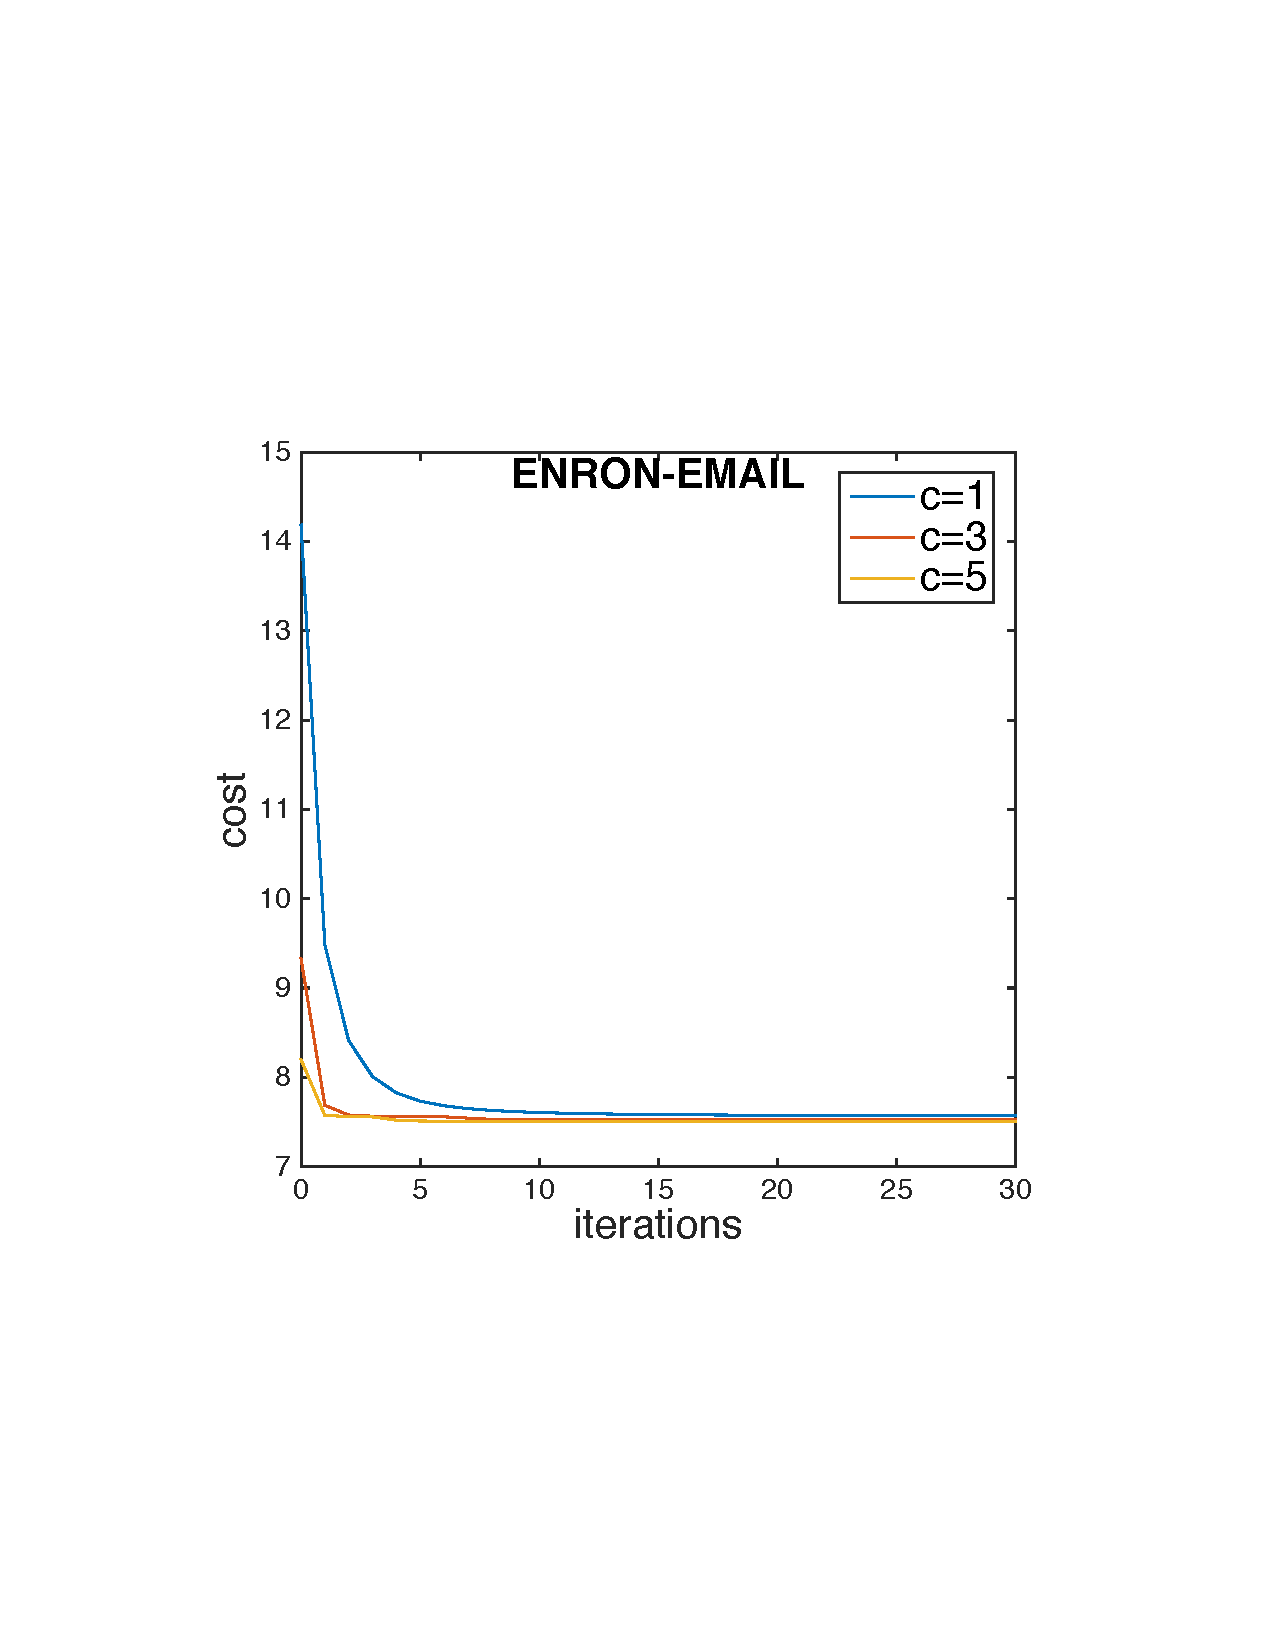
\includegraphics[width=0.49\textwidth]{figures/conv/enron-email.pdf}}
\subcaptionbox*{}{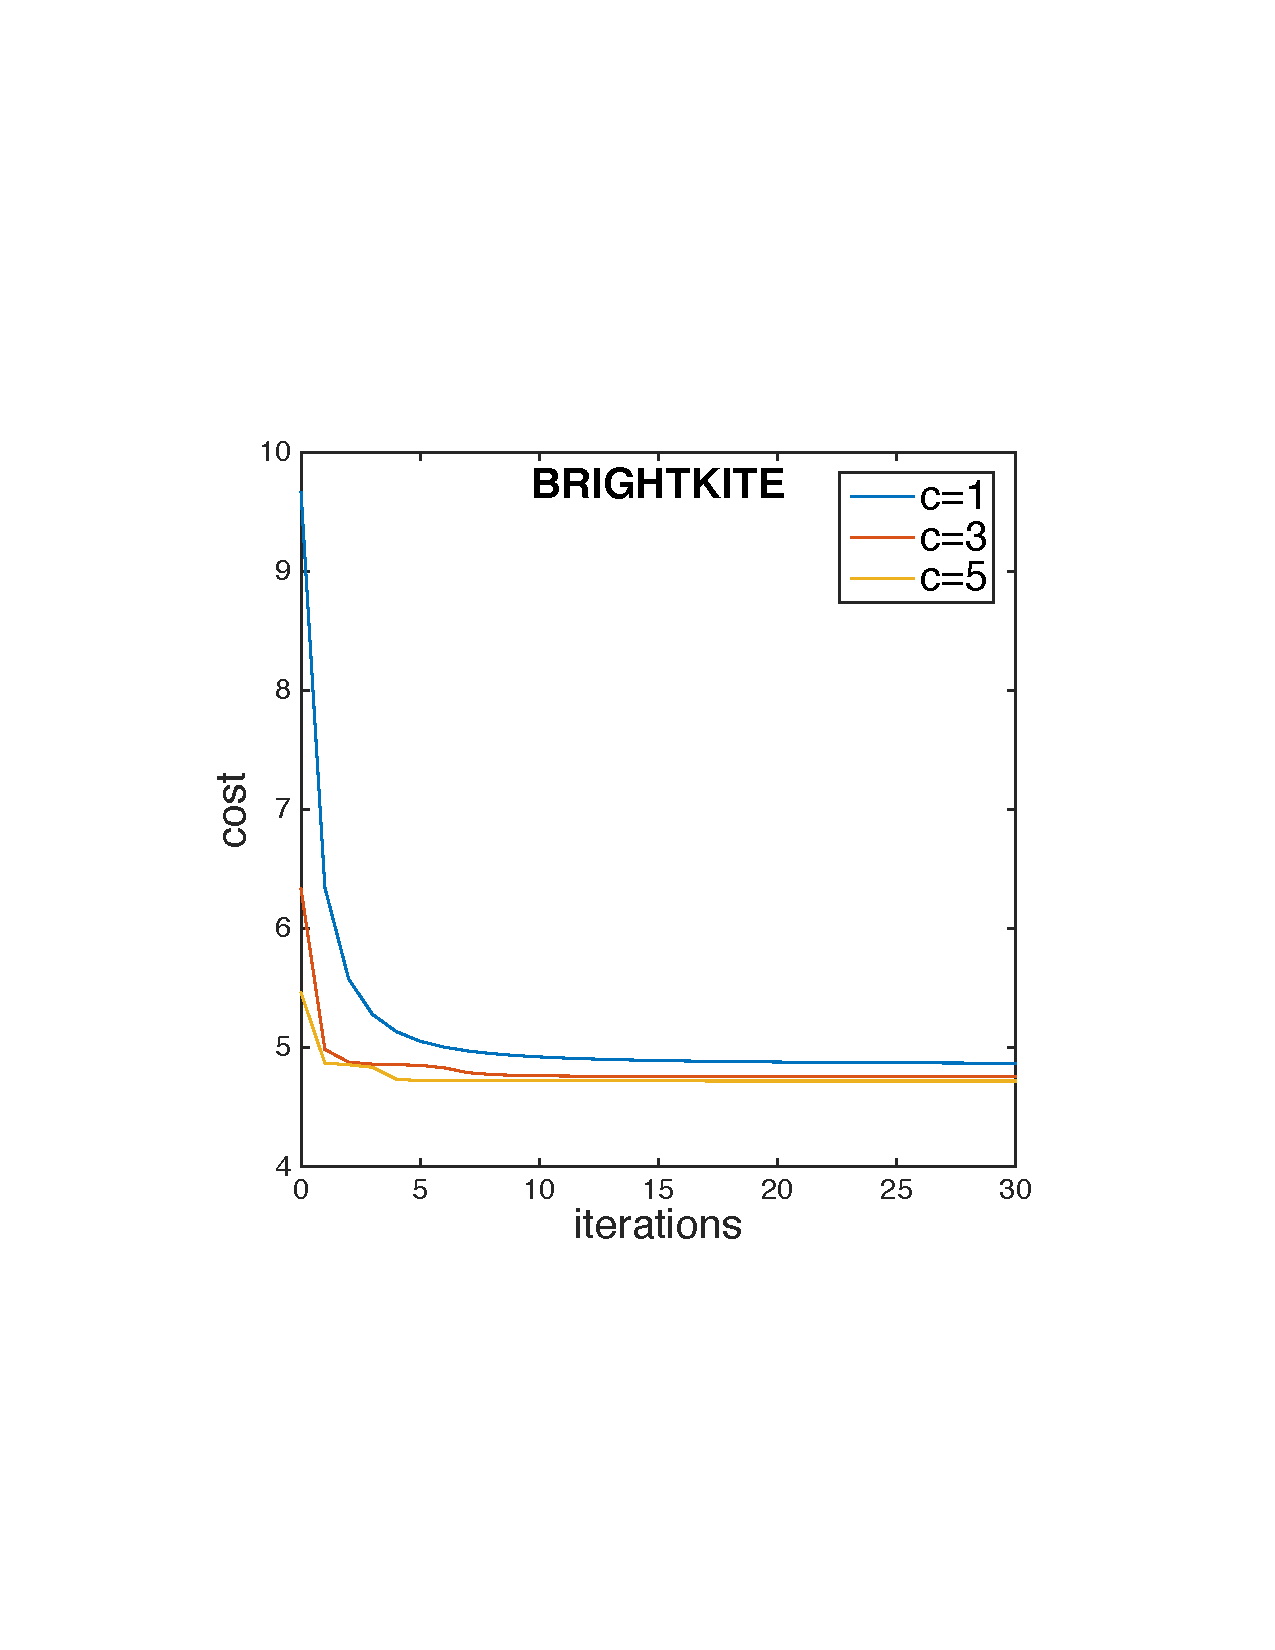
\includegraphics[width=0.49\textwidth]{figures/conv/brightkite.pdf}}
\subcaptionbox*{}{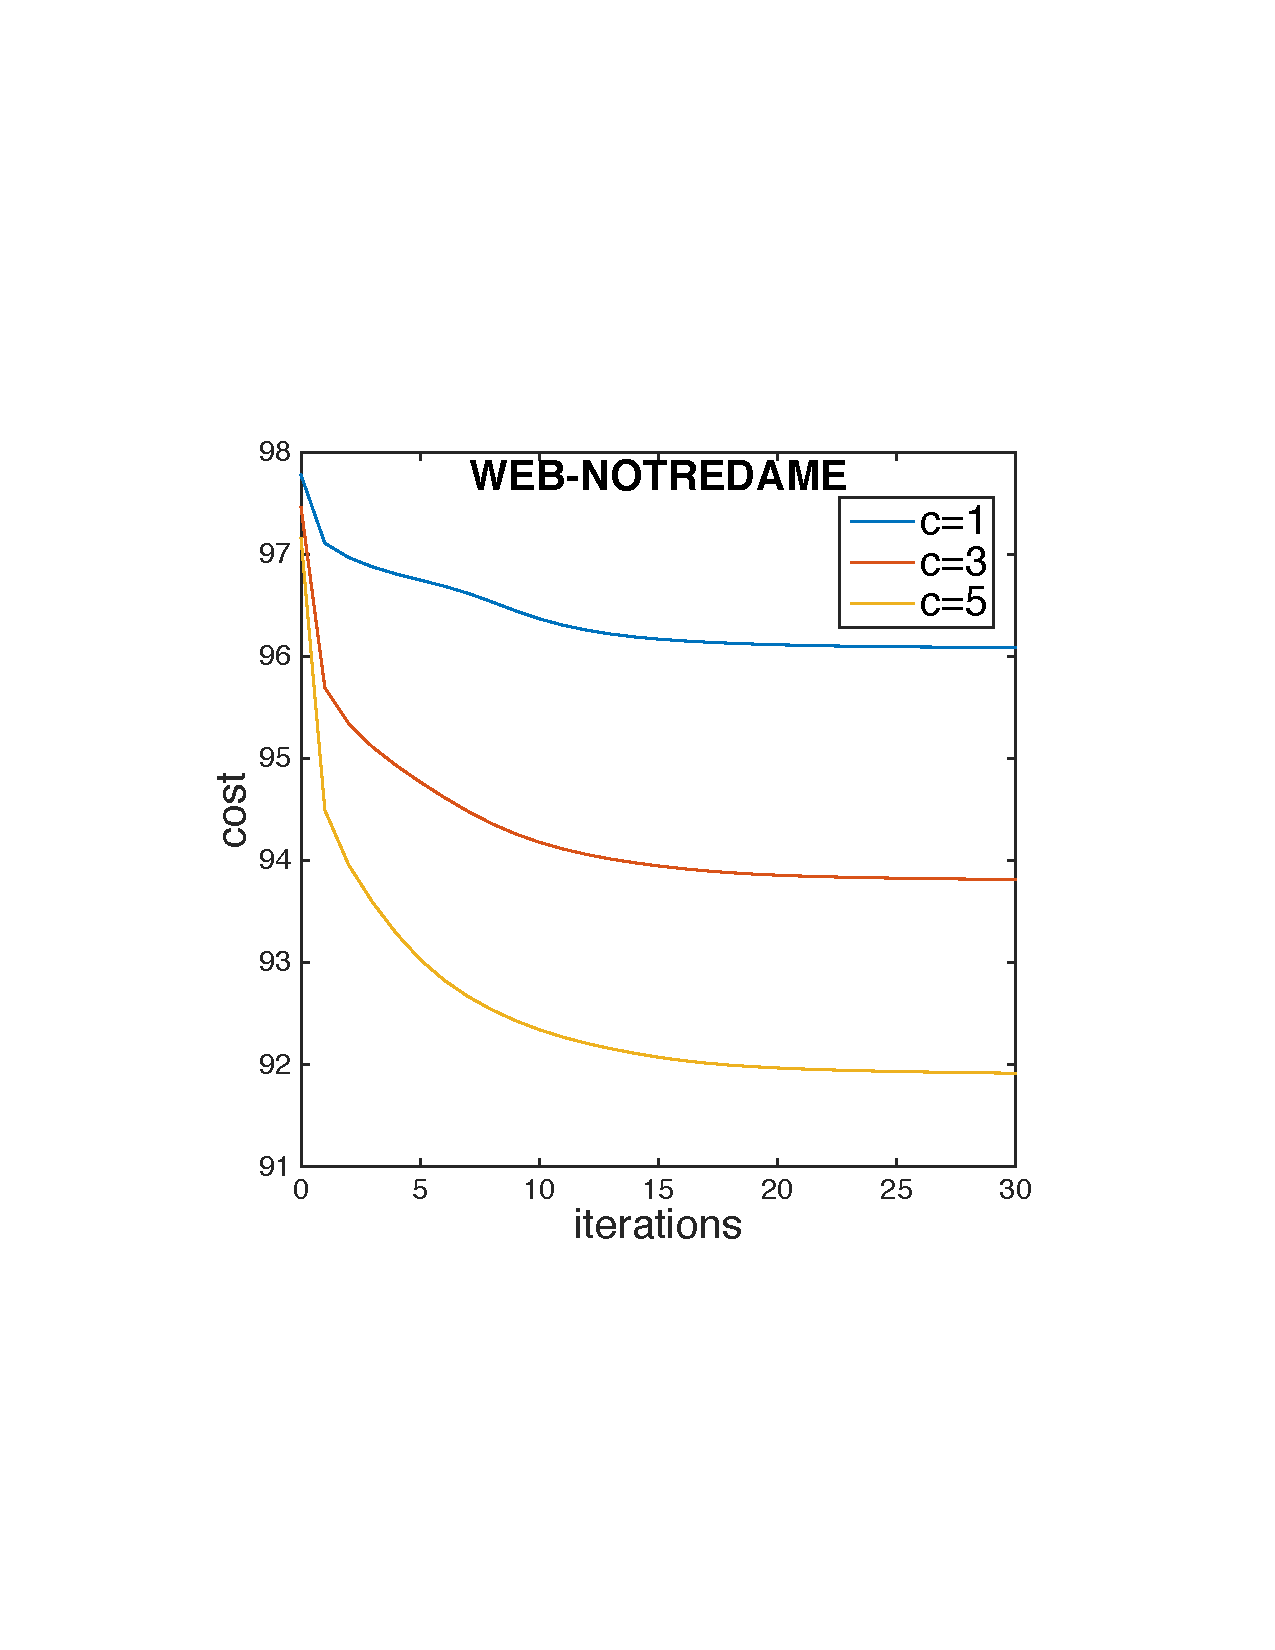
\includegraphics[width=0.49\textwidth]{figures/conv/web-notredame.pdf}}
\subcaptionbox*{}{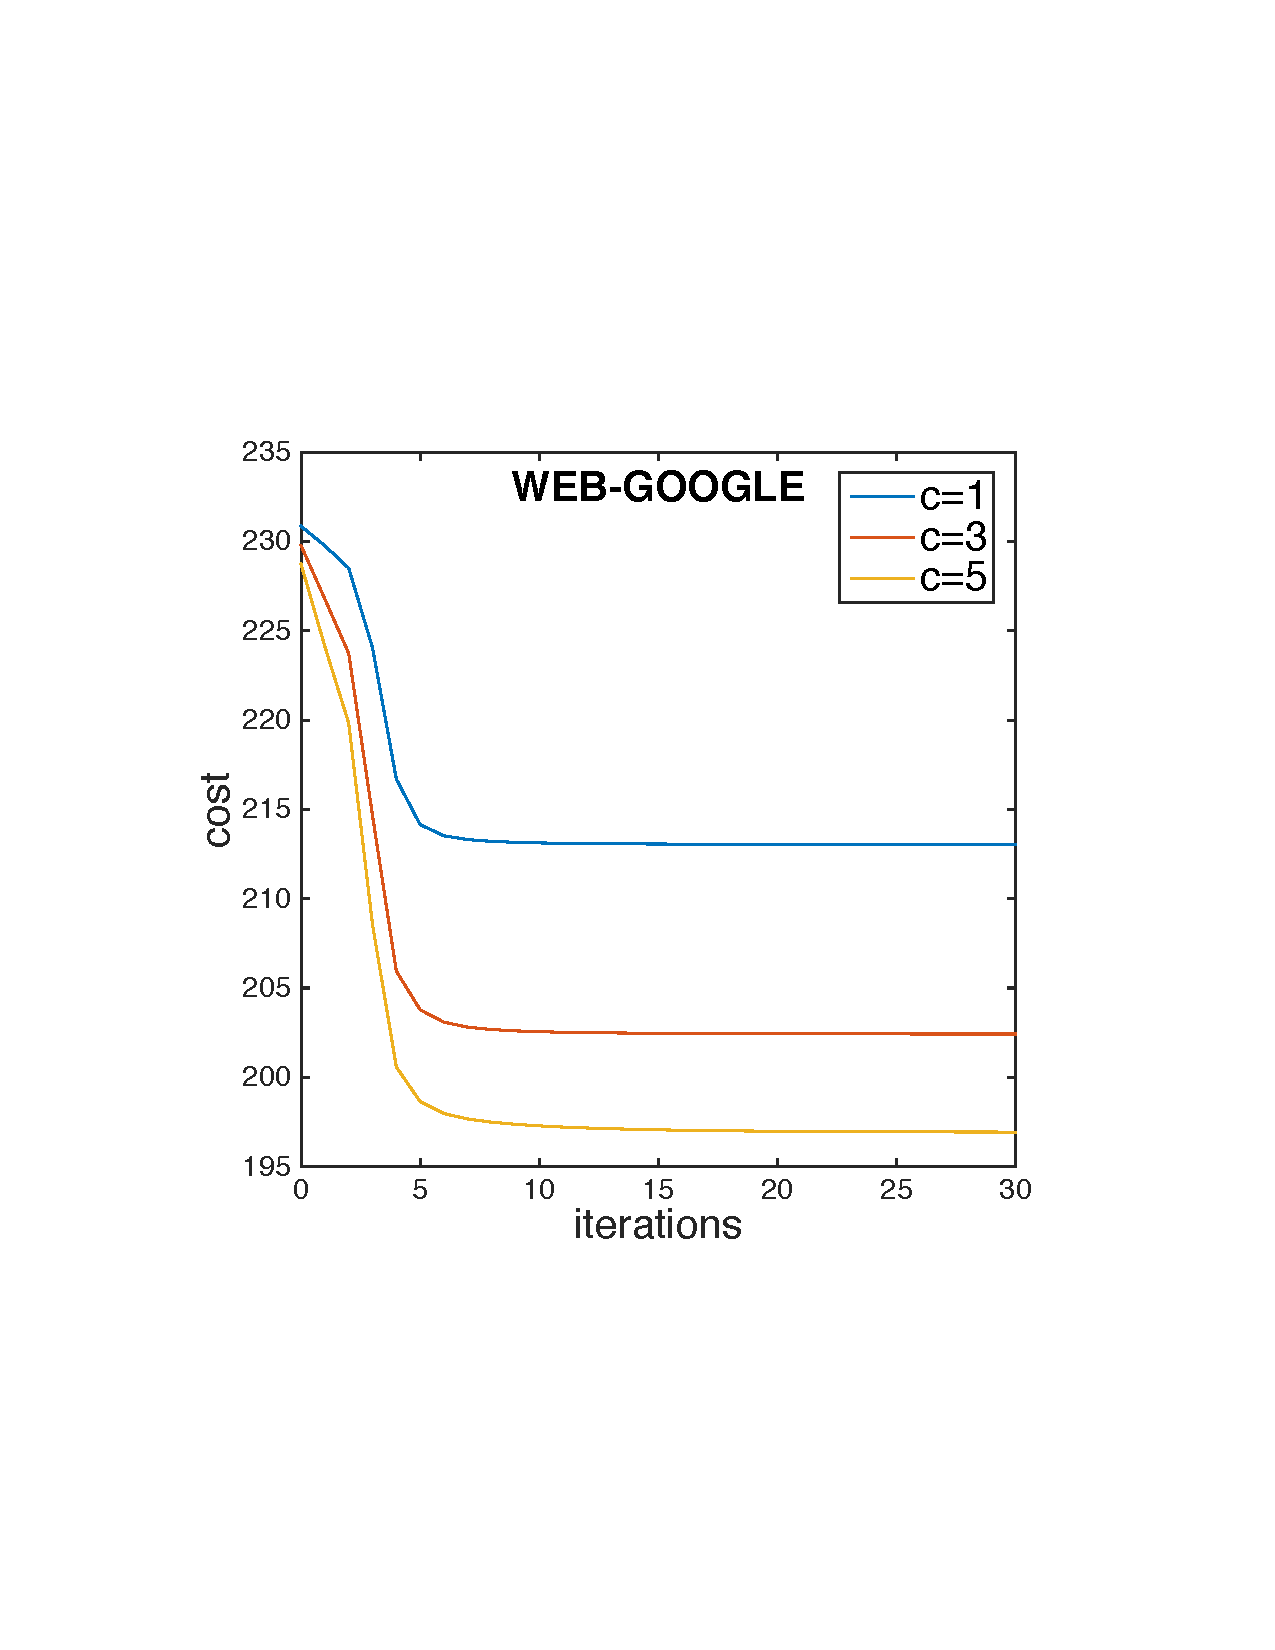
\includegraphics[width=0.49\textwidth]{figures/conv/web-google.pdf}}
\caption{\scriptsize The cost of intermediate $c$-schedules at iterations of \algonameapx  according to $\Sample$.}\label{fig:conv}
\end{figure}







Next, we extract the $1$-schedules  output by \algonameapx, and compare its cost to four other natural schedules: \texttt{unif}, \texttt{outdeg}, \texttt{indeg}, and \texttt{totdeg} that probe each node, respectively, uniformly, proportional to its out-degree, proportional to its in-degree, and proportional to number of incident edges. Note that for undirected graphs \texttt{outdeg}, \texttt{indeg}, and \texttt{totdeg} are essentially the same schedule. 

To have a fair comparison among the costs of these schedules and \algonameapx, we calculate their costs according to 10  independent samples, $\Sample_1,\ldots,\Sample_{10}$ that satisfy \eqref{eq:samp_cond}, and compute the average. The results are shown in Table~\ref{table:compare}, and show that \algonameapx outperforms the other four schedules.


%(i) \texttt{uniform} schedule, (ii) \texttt{outdeg} schedule that probes each node proportional to its out-degree, (iii) \texttt{indeg} schedule that probes each node proportional to its in-degree, and (iv) \texttt{totdeg} (note that for undirected graphs \texttt{outdegree} and \texttt{indegree} are the same). We compared the cost of these schedules according to another sample $\Sample'$ that satisfies the condition in Lemma~\ref{lem:chernoffcost}, and the results are shown in Table~\ref{table:compare}; numbers are obtained by averaging the 10 runs over 10 different sample $\Sample'$s.

\begin{table}[ht]
\centering
\resizebox{\columnwidth}{!}{
\caption{\scriptsize Comparing the costs of 5 different 1-schedules.}
\label{table:compare}
\begin{tabular}{lrrrrr}
\toprule
Dataset       & \algonameapx & \texttt{uniform} & \texttt{outdeg} & \texttt{indeg} & \texttt{totdeg} \\ 
\midrule
Enron-Email   &       7.55 & 14.16 & 9.21 & 9.21 & 9.21                  \\ 
Brightkite    &       4.85 & 9.64 & 6.14 & 6.14 & 6.14                  \\ 
web-Notredame &       96.10 & 97.78 & 97.37 & 97.43 & 97.40             \\ 
web-Google    &       213.15 & 230.88 & 230.48 & 230.47 & 230.47       \\
\bottomrule
\end{tabular}
}
\end{table}



% --------------------------------------------------
% --------------------------------------------------
% --------------------------------------------------
\subsubsection{A Test on Convergence to  Optimal Schedule}\label{sec:example}
Here, we present an example for which we know the optimal schedule, and moreover, the optimal schedule is unique. Therefore, we use this example to investigate further the convergence of \algonameapx. In particular, we would like to see how close the \algonameapx output is to the optimal schedule, regarding (i) different initial schedules, $\sched^0$ (which we let to be uniform), and (ii) samples $\Sample$'s  obtained during time intervals of different lengths.

Suppose $G=(V,E)$ is the complete graph where $V=[n]$. Let $\sys=(\family, \pi)$ for  $\family = \{S \in 2^{[n]} \mid 1 \leq|S| \leq 2\}$, and $\pi(S)=\frac{1}{|\family|}$. It is easy to see that $\cost_\theta(\sched)$ is a symmetric function, and thus, the uniform schedule is optimal. Moreover, by Corollary~\ref{corol:convexity} the uniform schedule is the only optimal schedule, since $\{v\} \in \family$ for every $v\in V$. Furthermore, we let $\theta=0.99$ to increase the sample complexity (as in Lemma~\ref{lem:chernoffcost}) and make it harder to learn the uniform/optimal schedule.

\begin{figure}[htbp]
	\subcaptionbox*{}{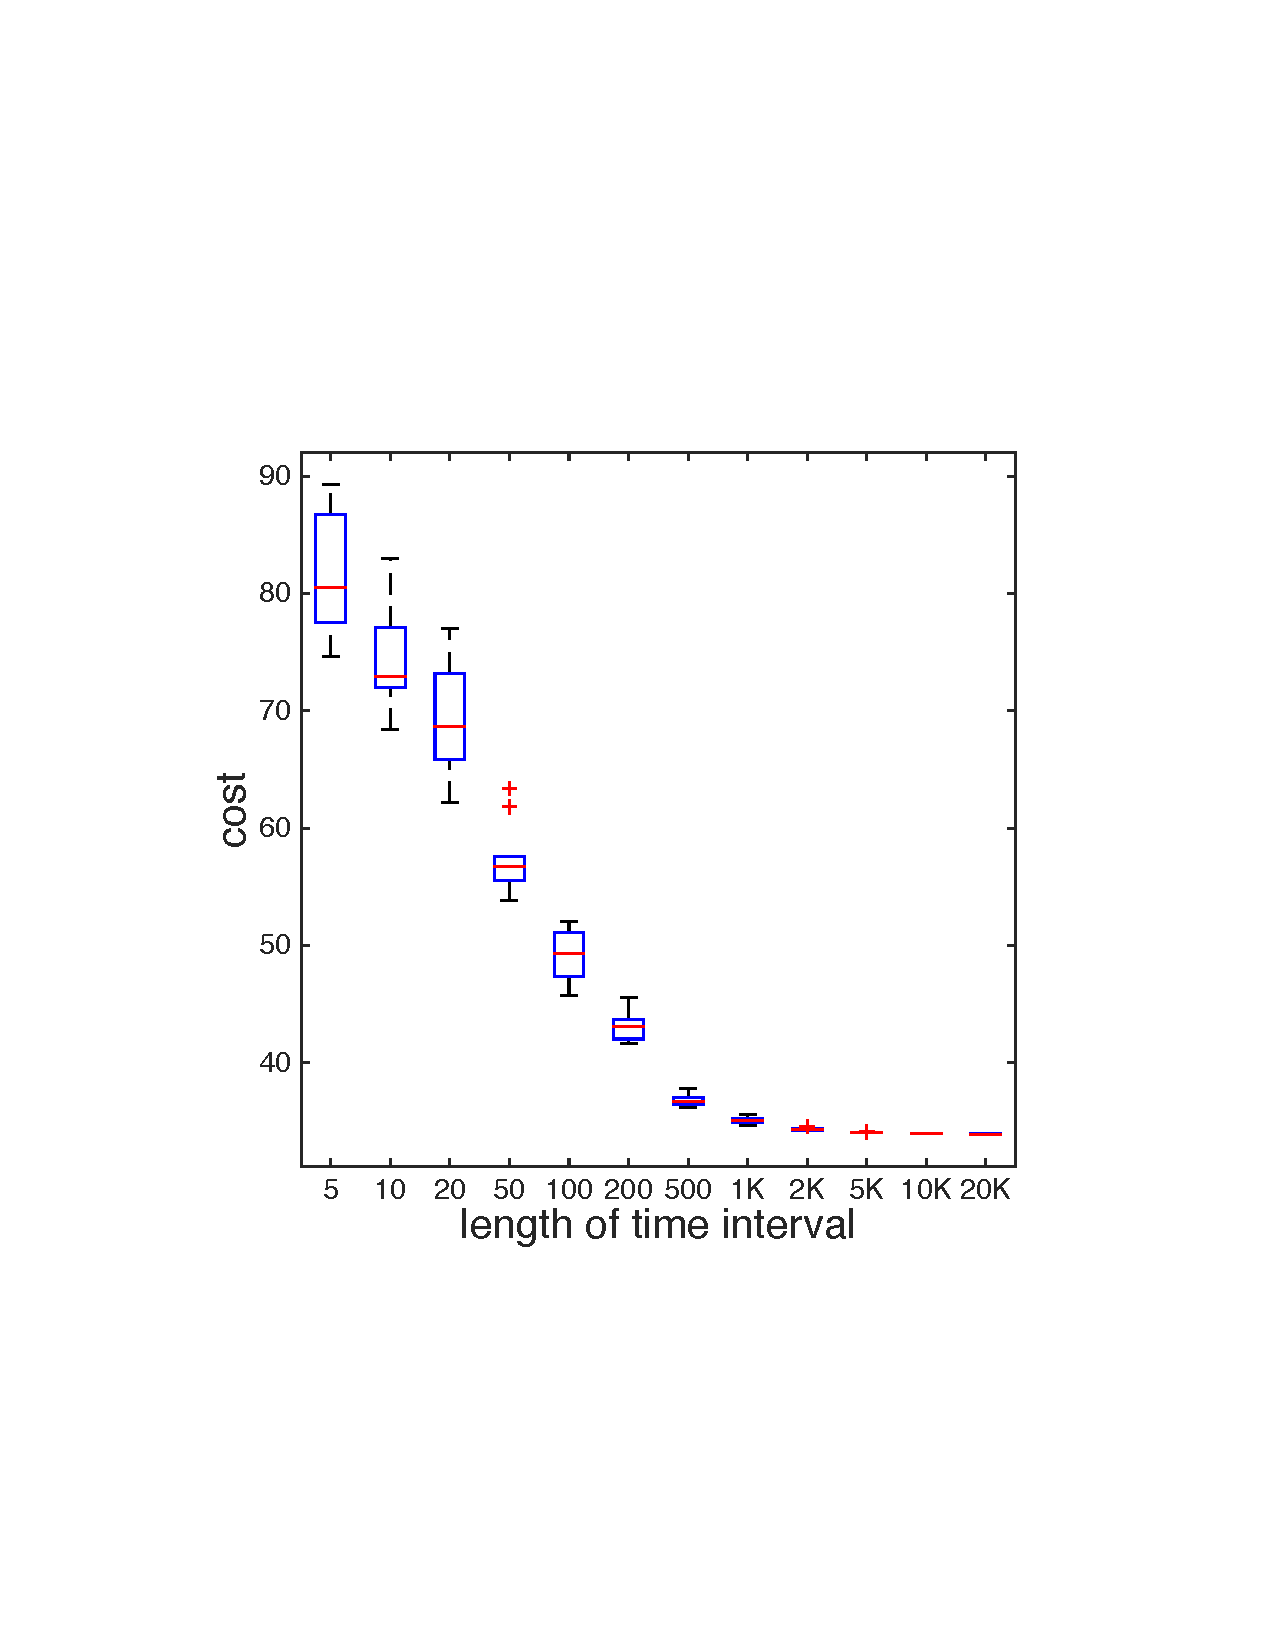
\includegraphics[width=0.49\textwidth]{figures/D100s/cost.pdf}}
	\subcaptionbox*{}{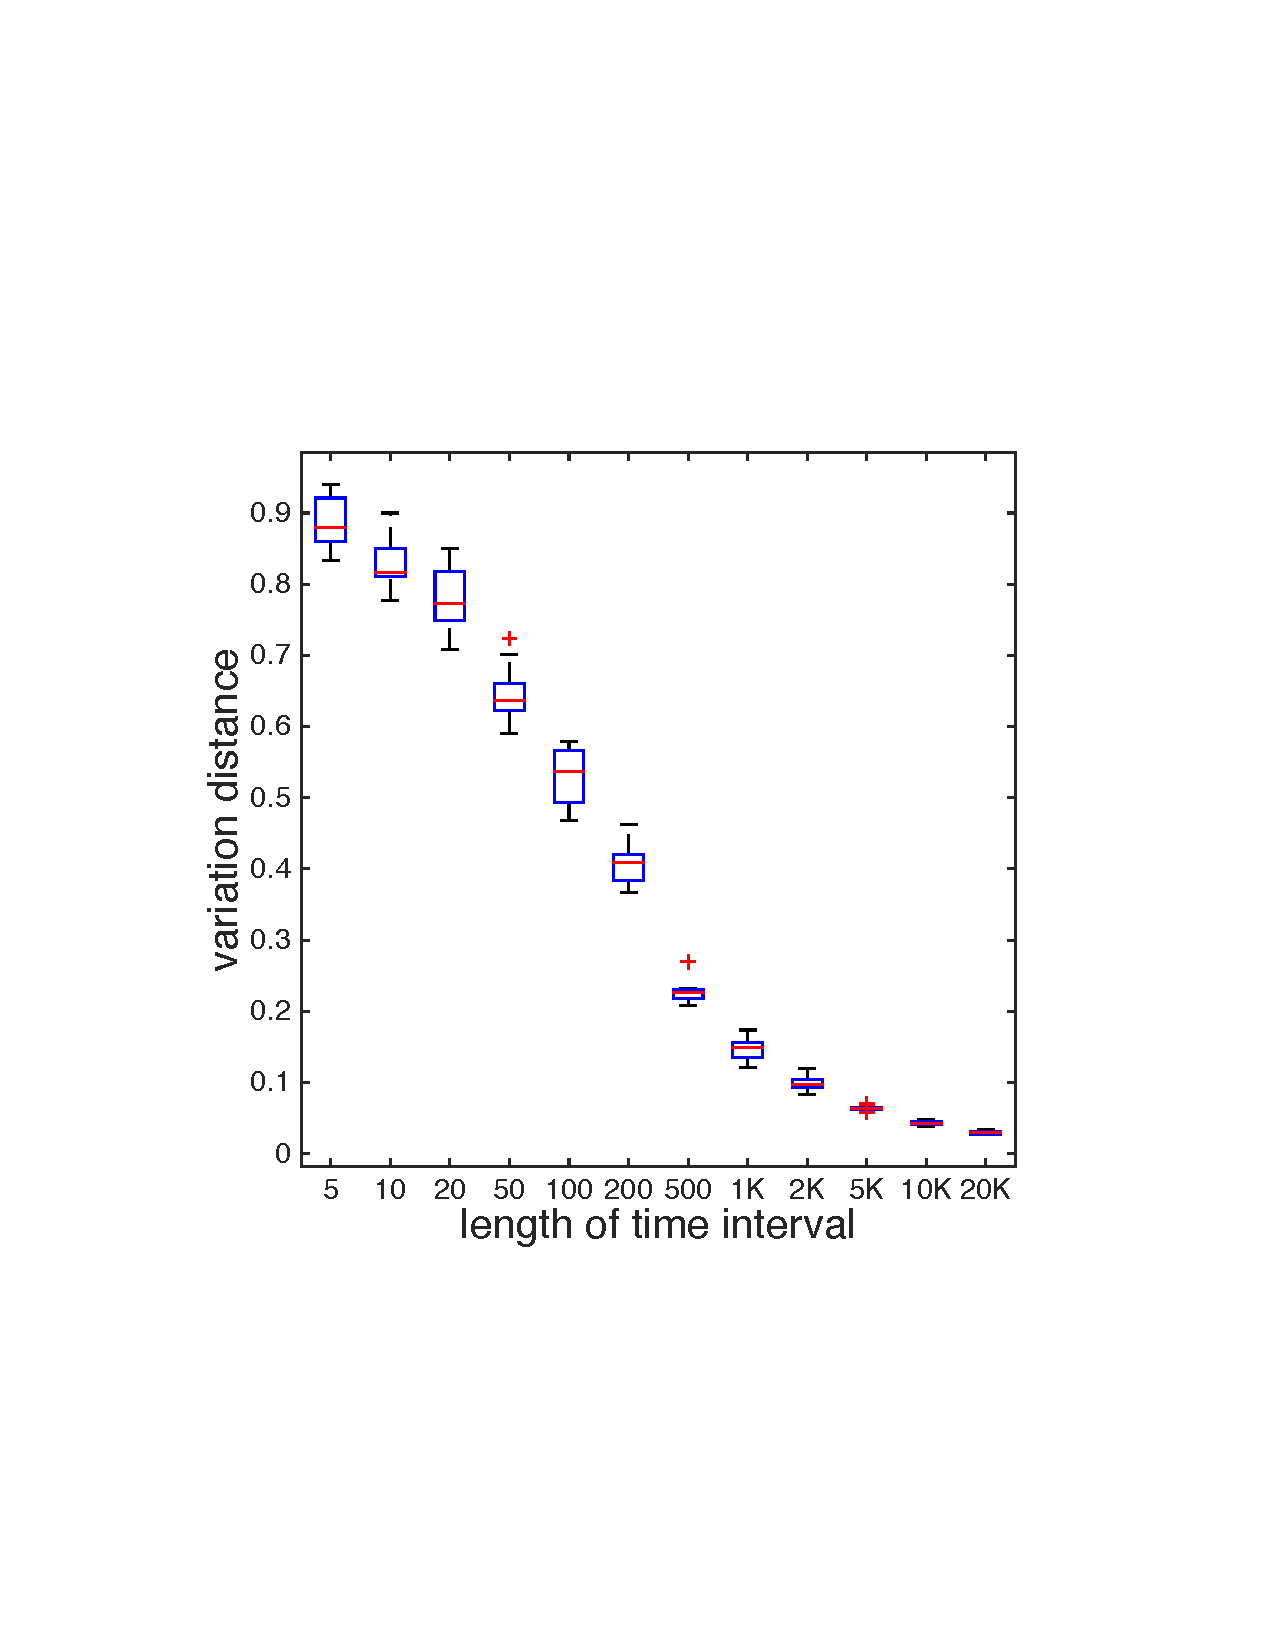
\includegraphics[width=0.49\textwidth]{figures/D100s/vardist.pdf}}
	\caption{\scriptsize The cost of \algonameapx outputs and their variation distance to the optimal schedule.} \label{fig:unique}
\end{figure}
In our experiments we run the \algonameapx algorithm, using (i) different \emph{random} initial schedules, and (ii) samples $\Sample$ obtained from time intervals of different lengths. For each sample, we run \algonameapx 10 times with 10 different random initial schedules, and compute the \textbf{exact} cost of each schedule, and its variation distance to the uniform schedule. Our results are plotted in Figure~\ref{fig:unique}, and as shown, by increasing the sample size (using longer time intervals of sampling) the output schedules gets very close to the uniform schedule (the variance gets smaller and smaller).

%-----------------------------------------------------------
%-----------------------------------------------------------
%-----------------------------------------------------------

\subsection{Dynamic Settings}\label{sec:dynset}
In this section, we present experimental results that show
 how our algorithm can adapt itself to the new situation.
Simulations are provided in Figure~\ref{figure:changes}: for each graph, we
start by following an 1-optimal schedule in the graph. At the beginning of each
``gray'' time interval, the labels of the nodes are permuted randomly, to impose
great disruptions in the system. Following that, at
the beginning of each ``green'' time interval our algorithm starts gathering
samples of $\sys$. Then, \algonameapx computes the schedule for the new sample, using 50 rounds of iterations, and starts probing. The length of each colored time
interval is $R = \frac{3(\log(n)+\log(2))}{\epsilon^2(1-\theta)}$, $\epsilon=0.5$, motivated by
Theorem~\ref{thm:approx_sample}.

%\todo[ahmad]{for $\epsilon=0.1$ and without making nodes generate up to 10: running}

%and other intervals (three time intervals before, between, and after the colored time intervals) have length $10R$. Also, for sake of illustration, we assumed at each time step each node $i$ may generated up to 10 items (each having a chance of $\pi_i$ to be generated). Thus, the number of generated items at each node is a binomial random variable with parameters 10 and $\pi$.
%Note that we start the generating process at time 0. Hence, during the first few time steps the load of the generating process increases.

Since the cost function is defined asymptotically (and explains the asymptotic behavior of the system in response to a schedule), in  Figure~\ref{figure:changes} we plot the load of the system $L_\theta(t)$ over the time (blue), and the \emph{average} load in the normal and perturbed time intervals (red). Based on this experiment, and as shown in Figure~\ref{figure:changes}, after adapting to the new schedule, the effect of the disruption caused by the perturbation disappears immediately. Note that when the difference between the optimal cost and any other schedule is small (like web-Notredame), the jump in the load will be small (e.g. as shown in Figure~\ref{fig:conv}), the cost of the initial schedule for web-Notredame is very close the optimal cost (obtained after 30 iteration).

%Based on our experiments, shown in Figure~\ref{figure:changes}, we observe that (i) a sample gathered during a very short time interval suffices to minimize the load (and therefore the cost) of the generating process, and (ii) after adapting to the new schedule, the effect of the perturbation disappears immediately (see the Section~\ref{sec:dynamic} for theoretical upper bound). Finally, note that for each time $t$, we plot the loads $L_\theta(t)$, and not the cost function. This is because the load is what we can observe (which is a draw of random variables $L_\theta(t)$), as the cost function is the expected value of these random variables averaged over the time, and it explains  the asymptotic behavior of the system.



\begin{figure}
%  \centering
  \subcaptionbox*{}{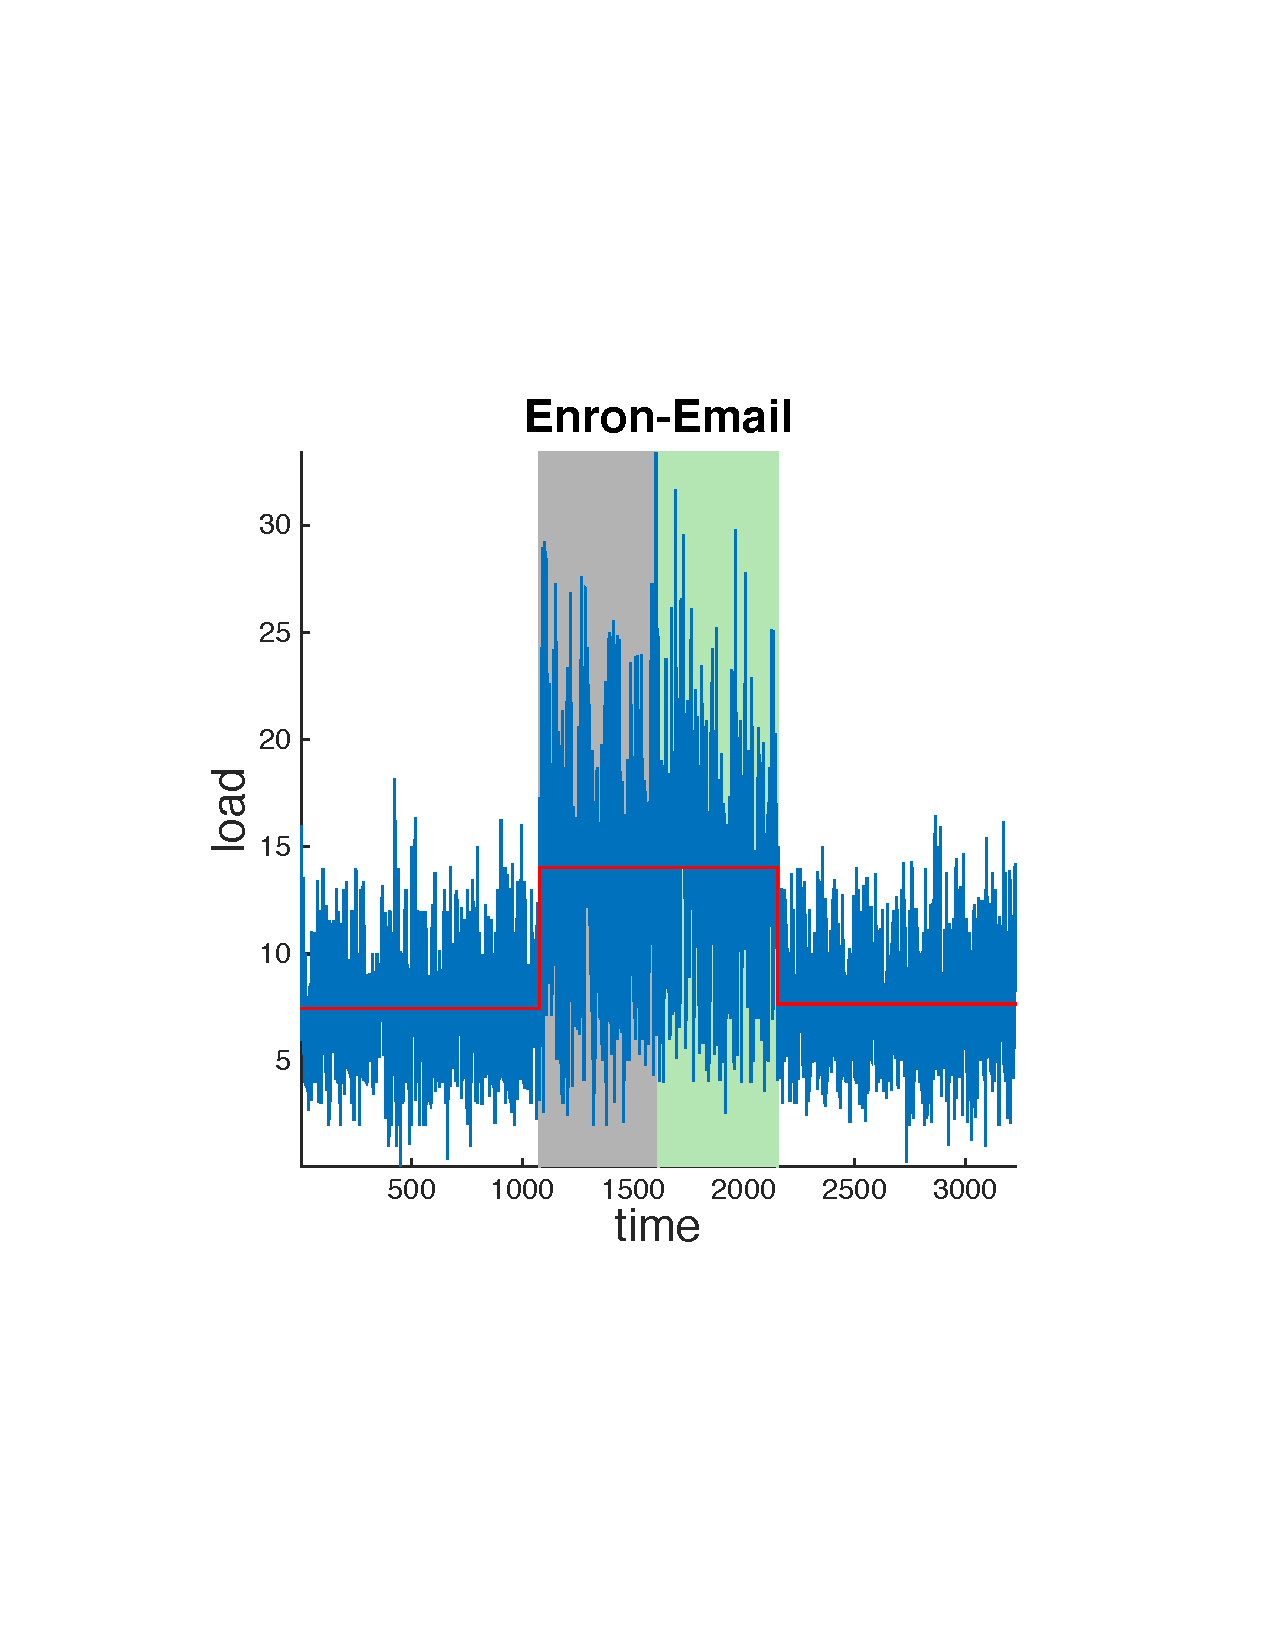
\includegraphics[width=0.49\textwidth]{figures/change/enron.pdf}} %\hspace{1em}%
  \subcaptionbox*{}{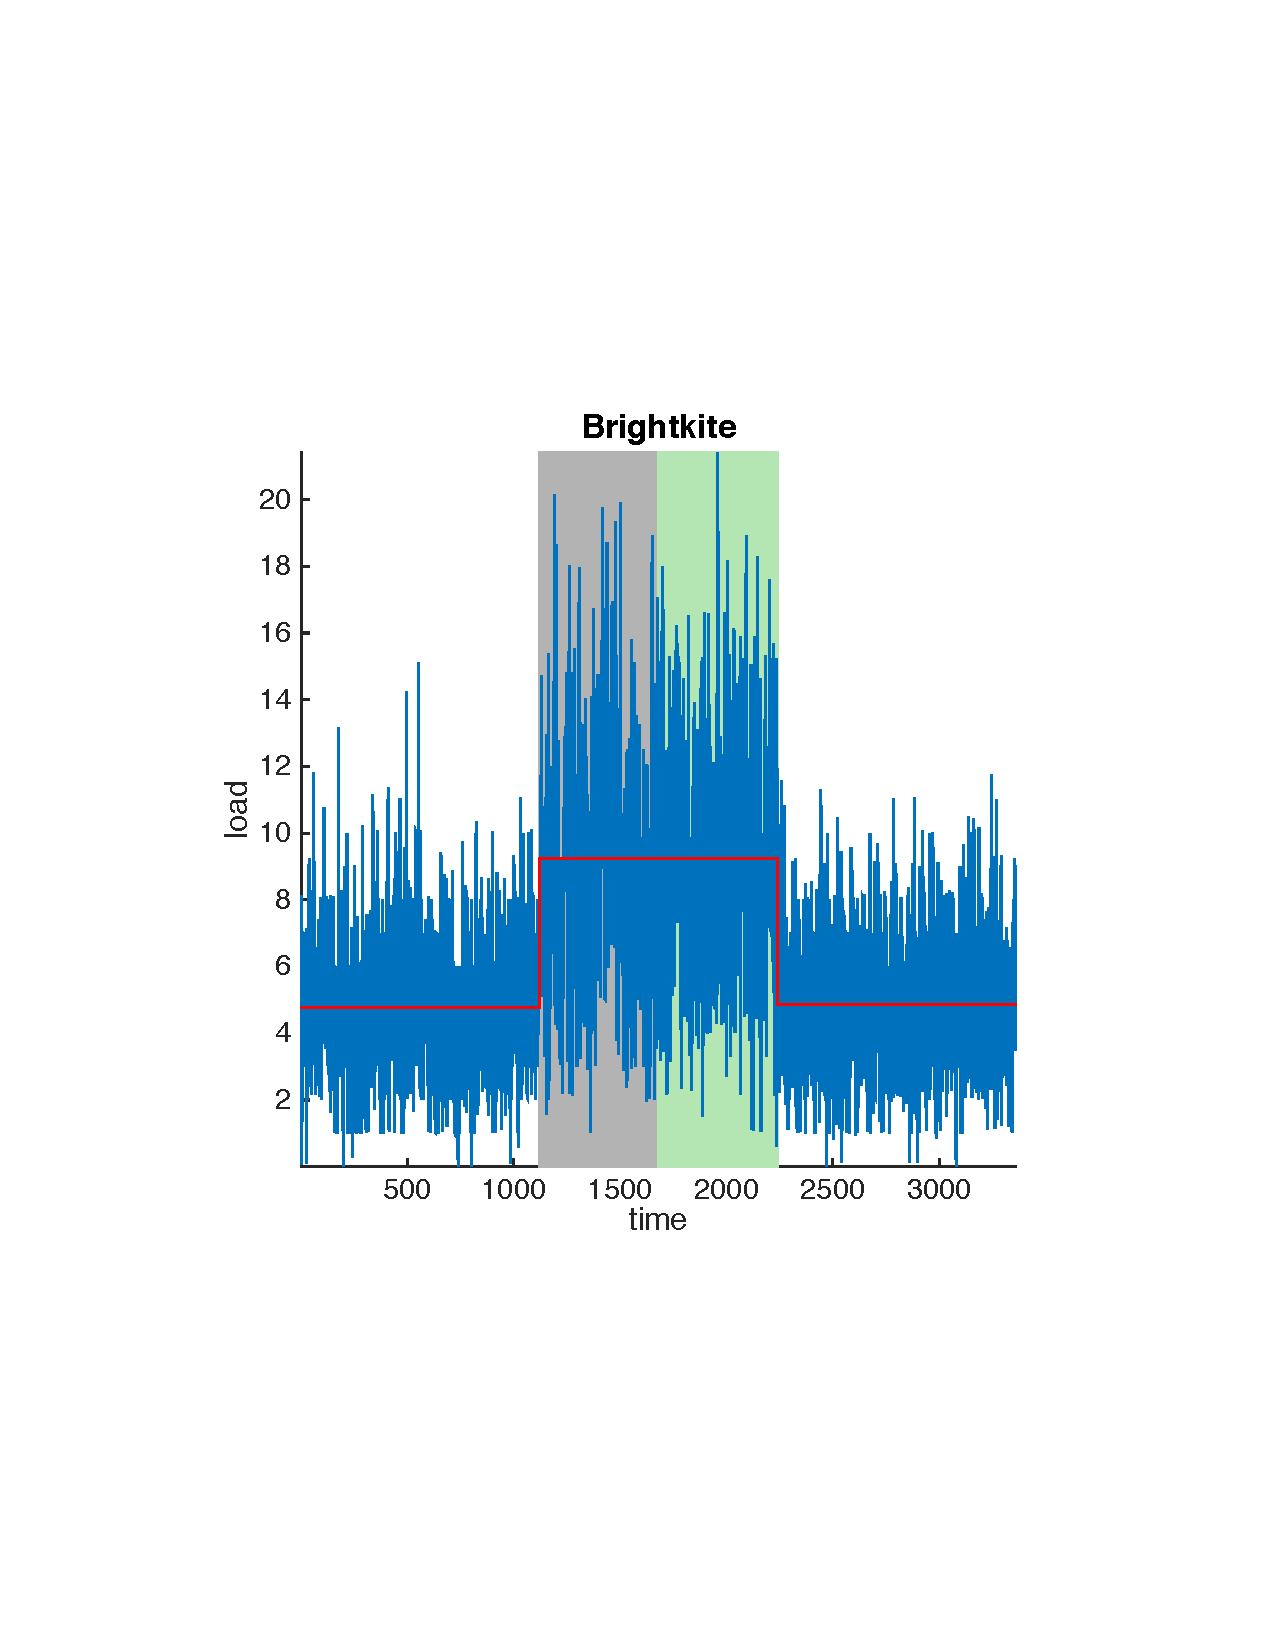
\includegraphics[width=0.49\textwidth]{figures/change/brightkite.pdf}} %\hspace{1em}
%  \subcaptionbox{Epinion\label{fig:change:epinion}}{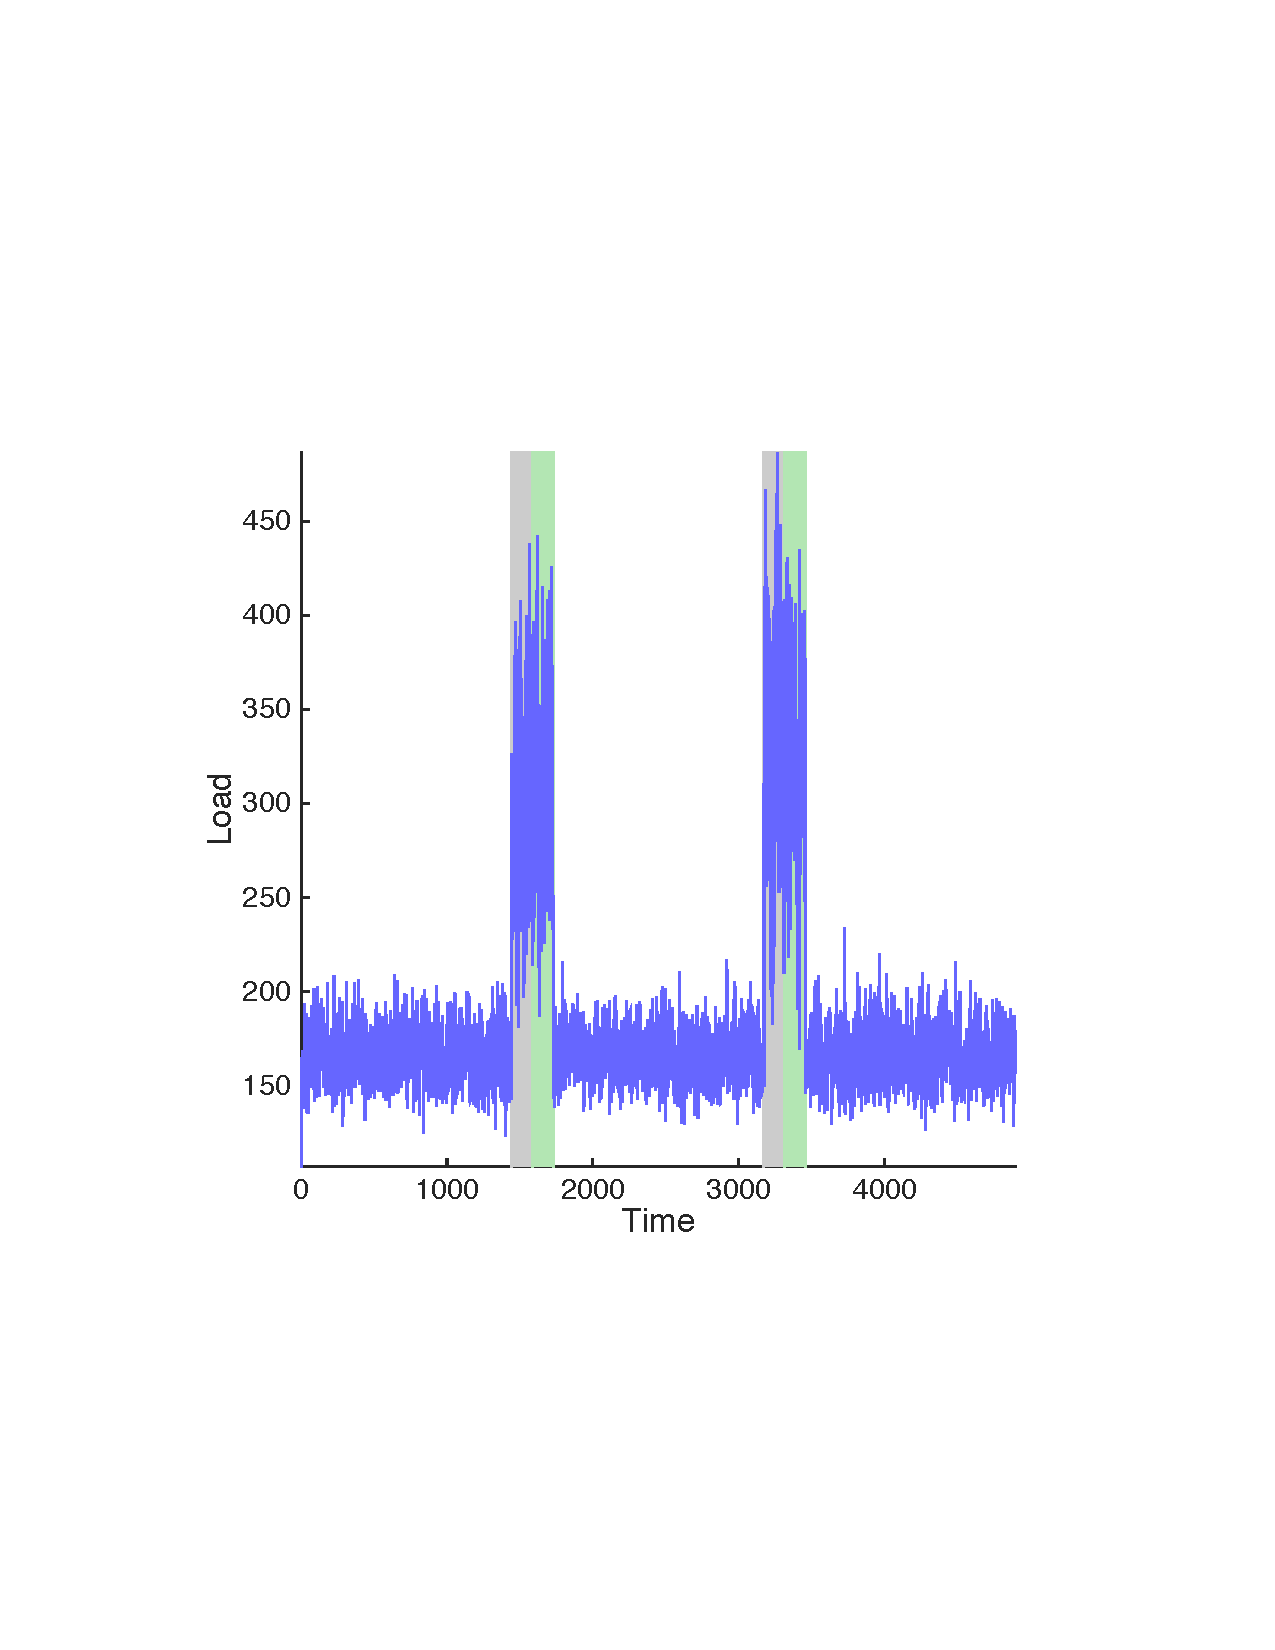
\includegraphics[width=0.3\textwidth]{figures/change/epinion.pdf}}\\ %\hspace{1em}\\
  \subcaptionbox*{}{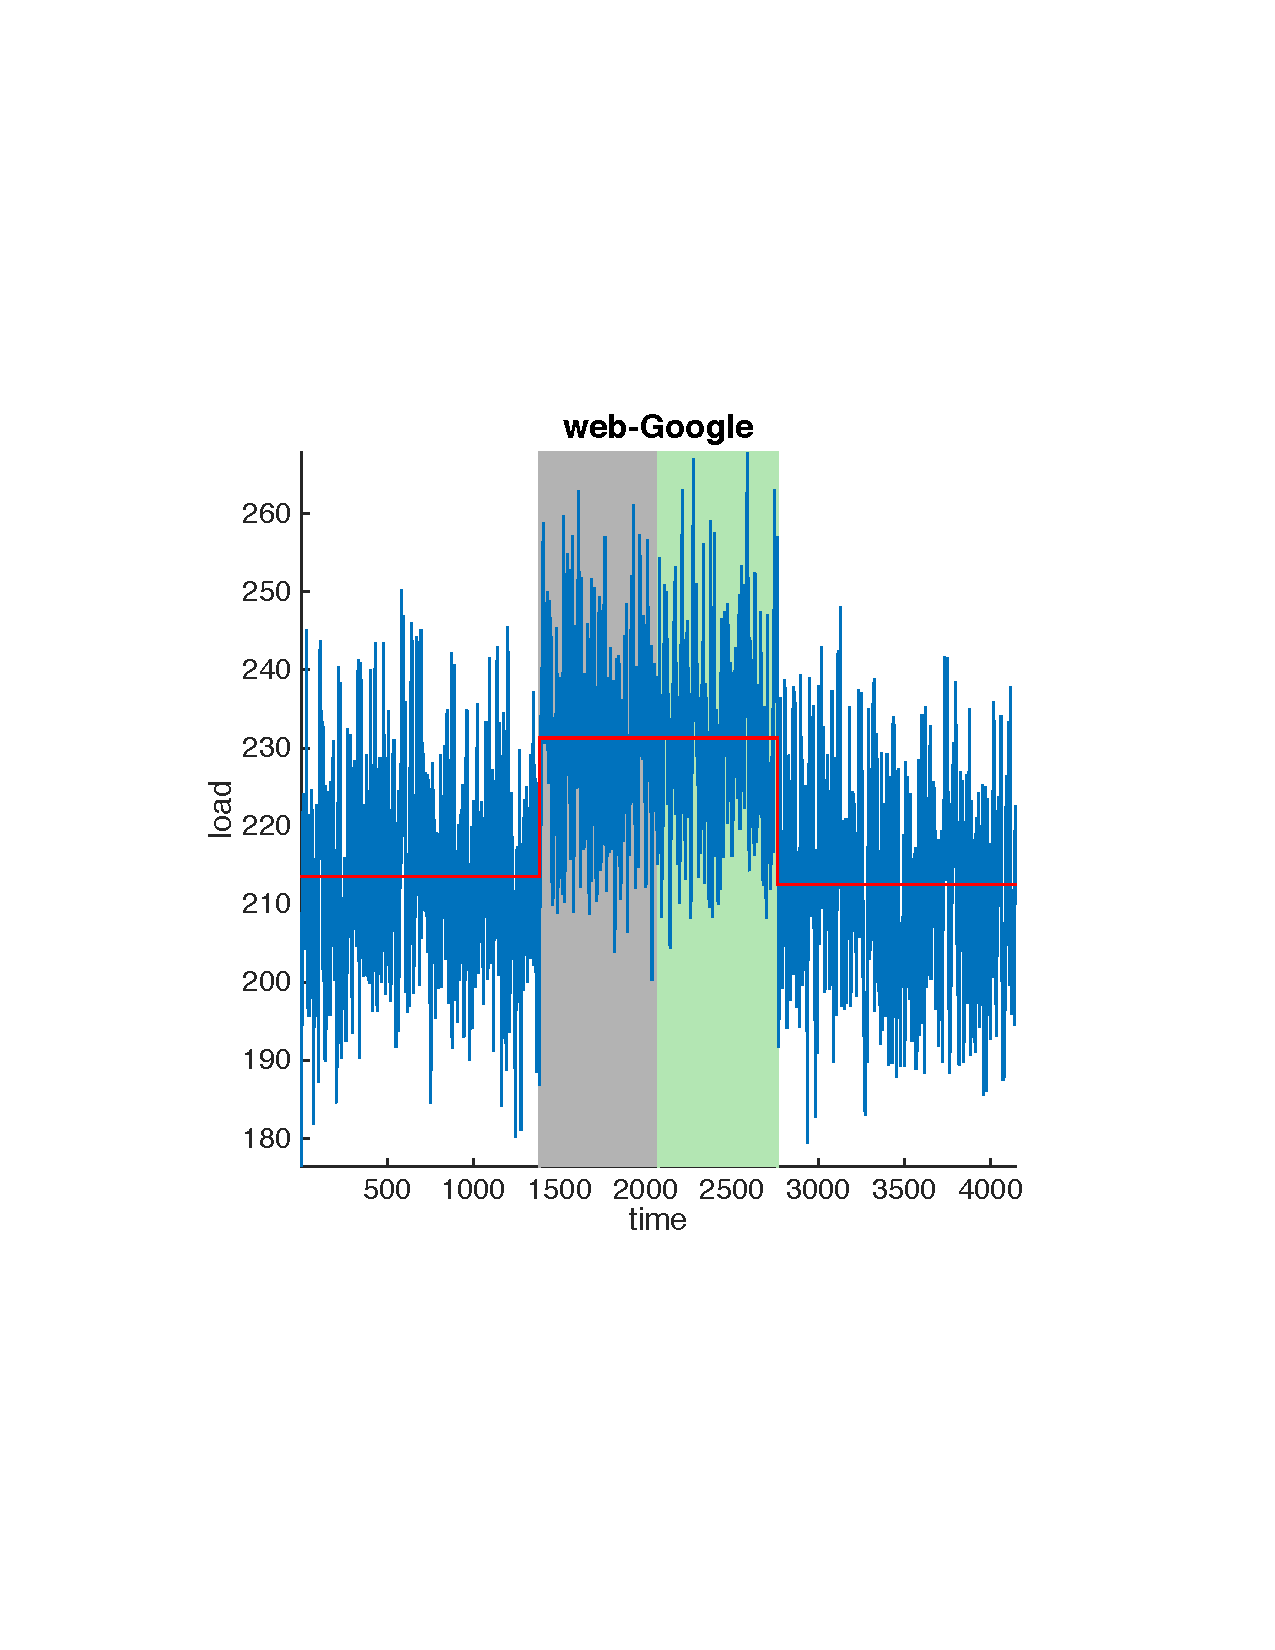
\includegraphics[width=0.49\textwidth]{figures/change/google.pdf}} %\hspace{1em}
  \subcaptionbox*{}{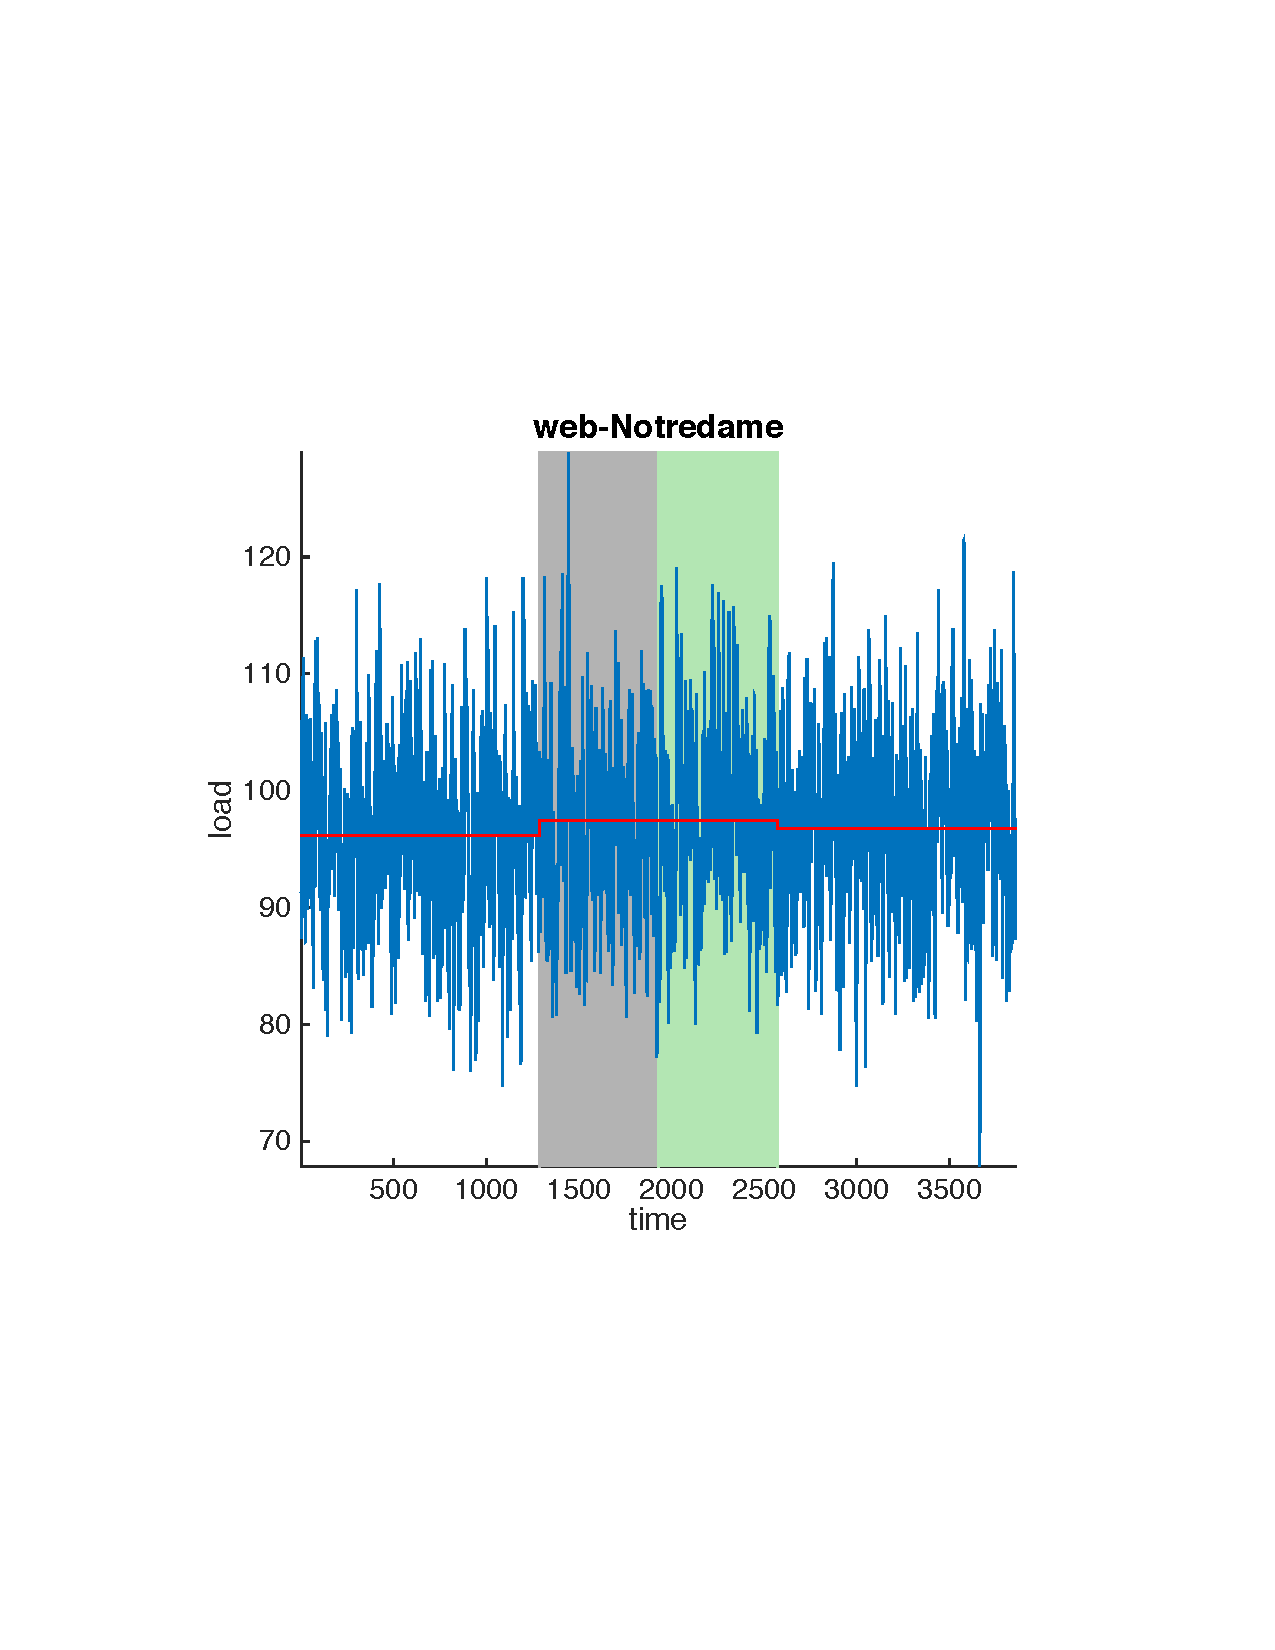
\includegraphics[width=0.49\textwidth]{figures/change/notredame.pdf}} %\hspace{1em}
  \caption{\scriptsize Perturbation, Sampling, and Adapting (For details see Section~\ref{sec:dynset}).}\label{figure:changes}
\end{figure}



\section{Conclusions}\label{sec:concl}

We formulate and study the $(\theta,c)$-Optimal Probing Schedule Problem,
which requires to find the best probing schedule that allows an observer to find
most pieces of information recently generated by a process $\sys$ by probing a
limited number of nodes at each time step.

We design and analyze an algorithm, \algoname, that can solve the problem
optimally if the parameters of the process $\sys$ are known, and then design a
variant that computes a high-quality approximation of the optimum schedule when
only a sample of the process is available. We also show that \algoname can be
adapted to the MapReduce framework of computation, which allows us to scale up
to networks with million of nodes. The results of experimental evaluation on a
variety of graphs and generating processes show that \algoname and its variants
are very effective in practice.

Interesting directions for future work include \ldots
\todo[all]{Need a couple of lines for future directions}


\section{Acknowledgements}
This work was supported by NSF grant IIS-1247581 and NIH grant R01-CA180776.

\bibliographystyle{abbrvnat}
\bibliography{catchRef}
%\setlength{\bibsep}{4pt}
%\fontsize{9}{10.2}
%\selectfont
\begin{thebibliography}{41}
\providecommand{\natexlab}[1]{#1}
\providecommand{\url}[1]{\texttt{#1}}
\expandafter\ifx\csname urlstyle\endcsname\relax
  \providecommand{\doi}[1]{doi: #1}\else
  \providecommand{\doi}{doi: \begingroup \urlstyle{rm}\Url}\fi

\bibitem[Agumbe~Suresh et~al.(2012)Agumbe~Suresh, Stoleru, Denton, Zechman, and
  Shihada]{AgumbeSuresh2012}
M.~Agumbe~Suresh, R.~Stoleru, R.~Denton, E.~Zechman, and B.~Shihada.
\newblock Towards optimal event detection and localization in acyclic flow
  networks.
\newblock ICDCN'12, 2012.


\bibitem[Boyd and Vandenberghe(2004)]{BoydV04}
S.~Boyd and L.~Vandenberghe.
\newblock \emph{Convex optimization}.
\newblock Cambridge university press, 2004.

\bibitem[Bright et~al.(2006)Bright, Gal, and
  Raschid]{adaptive-bright2006adaptive}
L.~Bright, A.~Gal, and L.~Raschid.
\newblock Adaptive pull-based policies for wide area data delivery.
\newblock \emph{ACM TODS}, 31\penalty0 (2):\penalty0 631--671, 2006.

\bibitem[Cataldi et~al.(2010)Cataldi, Di~Caro, and Schifanella]{Cataldi2010}
M.~Cataldi, L.~Di~Caro, and C.~Schifanella.
\newblock Emerging topic detection on {T}witter based on temporal and social
  terms evaluation.
\newblock MDMKDD'10, 2010.

\bibitem[Chen et~al.(2009)Chen, Wang, and Yang]{Chen2009}
W.~Chen, Y.~Wang, and S.~Yang.
\newblock Efficient influence maximization in social networks.
\newblock KDD'09, 2009.

\bibitem[Chen et~al.(2010)Chen, Wang, and Wang]{Chen2010}
W.~Chen, C.~Wang, and Y.~Wang.
\newblock Scalable influence maximization for prevalent viral marketing in
  large-scale social networks.
\newblock KDD'10, 2010.

\bibitem[Christakis and Fowler(2010)]{Christakis2010}
N.~A. Christakis and J.~H. Fowler.
\newblock {{S}ocial network sensors for early detection of contagious
  outbreaks}.
\newblock \emph{PLoS ONE}, 5\penalty0 (9):\penalty0 e12948, 2010.

\bibitem[Dasgupta et~al.(2007)Dasgupta, Ghosh, Kumar, Olston, Pandey, and
  Tomkins]{dasgupta2007discoverability}
A.~Dasgupta, A.~Ghosh, R.~Kumar, C.~Olston, S.~Pandey, and A.~Tomkins.
\newblock The discoverability of the web.
\newblock WWW'07, 2007.

\bibitem[Dean and Ghemawat(2008)]{dean2008mapreduce}
J.~Dean and S.~Ghemawat.
\newblock MapReduce: simplified data processing on large clusters.
\newblock \emph{CACM}, 51\penalty0 (1):\penalty0 107--113,
  2008.

\bibitem[Delaney(2009)]{Delaney2009}
A.~Delaney.
\newblock \emph{The Growing Role of News in Trading Automation}, Oct. 2009.
\newblock
  \url{http://www.machinereadablenews.com/images/dl/Machine_Readable_News_and_Algorithmic_Trading.pdf}.

\bibitem[Golovin et~al.(2010)Golovin, Faulkner, and Krause]{Golovin2010}
D.~Golovin, M.~Faulkner, and A.~Krause.
\newblock Online distributed sensor selection.
\newblock IPSN'10, 2010.

\bibitem[Hardy(1991)]{Hardy91}
G.~H. Hardy.
\newblock \emph{Divergent series}, volume 334.
\newblock Am.~Math.~Soc., 1991.

\bibitem[Hart and Murray(2010)]{Hart2010}
W.~Hart and R.~Murray.
\newblock Review of sensor placement strategies for contamination warning
  systems in drinking water distribution systems.
\newblock \emph{J. Water Resources Planning and Manag.},
  136\penalty0 (6):\penalty0 611--619, 2010.
\newblock \doi{10.1061/(ASCE)WR.1943-5452.0000081}.

\bibitem[Hope(2015)]{wallstreet2015}
B.~Hope.
\newblock How computers trawl a sea of data for stock picks.
\newblock \emph{The Wall Street Journal}, Apr. 1st 2015.

\bibitem[Horincar et~al.(2014)Horincar, Amann, and
  Arti{\`e}res]{onlineRef-horincar2014online}
R.~Horincar, B.~Amann, and T.~Arti{\`e}res.
\newblock Online refresh strategies for content based feed aggregation.
\newblock \emph{World Wide Web}, 1--35, 2014.

\bibitem[Jung et~al.(2011)Jung, Heo, and Chen]{jung2011irie}
K.~Jung, W.~Heo, and W.~Chen.
\newblock {IRIE}: Scalable and robust influence maximization in social
  networks.
\newblock \emph{arXiv:1111.4795}, 2011.

\bibitem[Kempe et~al.(2003)Kempe, Kleinberg, and Tardos]{Kempe2003}
D.~Kempe, J.~Kleinberg, and E.~Tardos.
\newblock Maximizing the spread of influence through a social network.
\newblock KDD'03, 2003.

\bibitem[Kempe et~al.(2005)Kempe, Kleinberg, and Tardos]{Kempe2005}
D.~Kempe, J.~Kleinberg, and E.~Tardos.
\newblock Influential nodes in a diffusion model for social networks.
\newblock ICALP'05, 2005.

\bibitem[Krause and Guestrin(2011)]{Krause2011}
A.~Krause and C.~Guestrin.
\newblock Submodularity and its applications in optimized information
  gathering.
\newblock \emph{ACM TIST}, 2\penalty0 (4):\penalty0
  32:1--32:20, 2011.

\bibitem[Krause et~al.(2008)Krause, Leskovec, Guestrin, VanBriesen, and
  Faloutsos]{Krause2008}
A.~Krause, J.~Leskovec, C.~Guestrin, J.~VanBriesen, and C.~Faloutsos.
\newblock Efficient sensor placement optimization for securing large water
  distribution networks.
\newblock \emph{J.~Water Resources Planning and Manag.},
  134\penalty0 (6):\penalty0 516--526, 2008.

\bibitem[Krause et~al.(2009)Krause, Rajagopal, Gupta, and Guestrin]{Krause2009}
A.~Krause, R.~Rajagopal, A.~Gupta, and C.~Guestrin.
\newblock Simultaneous placement and scheduling of sensors.
\newblock IPSN'09, 2009.

\bibitem[Krause et~al.(2011)Krause, Guestrin, Gupta, and
  Kleinberg]{Krause2011Kleinberg}
A.~Krause, C.~Guestrin, A.~Gupta, and J.~Kleinberg.
\newblock Robust sensor placements at informative and communication-efficient
  locations.
\newblock \emph{ACM TSN}, 7\penalty0 (4):\penalty0 31:1--31:33, 2011.

\bibitem[Kuhlman et~al.(2013)Kuhlman, Tuli, Swarup, Marathe, and
  Ravi]{Kuhlman2013}
C.~J. Kuhlman, G.~Tuli, S.~Swarup, M.~V. Marathe, and S.~S. Ravi.
\newblock Blocking simple and complex contagion by edge removal.
\newblock ICDM'13, 2013.

\bibitem[Latar(2015)]{latar2015robot}
N.~L. Latar.
\newblock The robot journalist in the age of social physics: The end of human
  journalism?
\newblock In \emph{The New World of Transitioned Media}, 65--80.
  Springer, 2015.

\bibitem[Leskovec et~al.(2007)Leskovec, Krause, Guestrin, Faloutsos,
  VanBriesen, and Glance]{Leskovec2007}
J.~Leskovec, A.~Krause, C.~Guestrin, C.~Faloutsos, J.~M. VanBriesen, and N.~S.
  Glance.
\newblock Cost-effective outbreak detection in networks.
\newblock KDD'07, 2007.

\bibitem[Li and Tang(2011)]{Li2011}
A.~Li and L.~Tang.
\newblock The complexity and approximability of minimum contamination problems.
\newblock TAMC'11, 2001.

\bibitem[Mathioudakis and Koudas(2010)]{Mathioudakis2010}
M.~Mathioudakis and N.~Koudas.
\newblock Twittermonitor: Trend detection over the {T}witter stream.
\newblock SIGMOD'10, 2010.

\bibitem[McKinney(2011)]{McKinney2011}
W.~McKinney.
\newblock \emph{Structured Data Challenges in Finance and Statistics}, 2011.
\newblock
  \url{http://www.slideshare.net/wesm/structured-data-challenges-in-finance-and-statistics}.

\bibitem[Mitzenmacher and Upfal(2005)]{MitzenmacherU05}
M.~Mitzenmacher and E.~Upfal.
\newblock \emph{Probability and Computing: Randomized Algorithms and
  Probabilistic Analysis}.
\newblock Cambridge University Press, 2005.

\bibitem[Oita and Senellart(2011)]{survey-oita2011deriving}
M.~Oita and P.~Senellart.
\newblock Deriving dynamics of web pages: A survey.
\newblock TWAW'11, 2011.

\bibitem[Ostfeld et~al.(2008)Ostfeld, Uber, Salomons, Berry, Hart, Phillips,
  Watson, Dorini, Jonkergouw, Kapelan, di~Pierro, Khu, Savic, Eliades,
  Polycarpou, Ghimire, Barkdoll, Gueli, Huang, McBean, James, Krause, Leskovec,
  Isovitsch, Xu, Guestrin, VanBriesen, Small, Fischbeck, Preis, Propato,
  Piller, Trachtman, Wu, and Walski]{BWSN2008}
A.~Ostfeld et al.
\newblock The battle of the water sensor networks ({BWSN}): A design challenge
  for engineers and algorithms.
\newblock \emph{J.~Water Resources Planning and Manag.},
  134\penalty0 (6):\penalty0 556--568, 2008.

\bibitem[Sia et~al.(2007)Sia, Cho, and Cho]{fast-sia2007efficient}
K.~C. Sia, J.~Cho, and H.-K. Cho.
\newblock Efficient monitoring algorithm for fast news alerts.
\newblock \emph{Knowledge and Data Engineering, IEEE Transactions on},
  19\penalty0 (7):\penalty0 950--961, 2007.

\bibitem[Tang et~al.(2014)Tang, Xiao, and Shi]{tang2014influence}
Y.~Tang, X.~Xiao, and Y.~Shi.
\newblock Influence maximization: Near-optimal time complexity meets practical
  efficiency.
\newblock \emph{arXiv:1404.0900}, 2014.

\bibitem[Wolf et~al.(2002)Wolf, Squillante, Yu, Sethuraman, and
  Ozsen]{wolf2002optimal}
J.~L. Wolf, M.~S. Squillante, P.~Yu, J.~Sethuraman, and L.~Ozsen.
\newblock Optimal crawling strategies for web search engines.
\newblock WWW'02, 2002.
\end{thebibliography}



% \appendix
% \section{Proof of Lemma 1}\label{app:proof}

 Let $i=i_{t, S}$ be an item. The probability that $i$ is still uncaught at time $t'$ is $(1-\p(S))^{c(t'-t)}$, and its freshness at $t'$ is $\theta^{t' - t}$. Therefore, $i$ imposes the load $\theta^{t'-t}$ to the system at time $t'$, with probability $(1-\p(S))^{c(t'-t)}$, and zero otherwise. Since the probability of $i_{t,S}$ being generated is $\pi(S)$ we have
\begin{align*}
 \cost{\p} &= \limsup_{t\rightarrow\infty}\frac{1}{t}\sum_{t'=0}^t\E(L_{\sys}(t')) = \limsup_{t\rightarrow \infty} \E\paran{L_{\sys}(t)} \\
 &=\lim_{t\rightarrow \infty} \sum_{S\in \F} \pi(S) \paran{1 + \theta\cdot(1-\p(S))^c + \ldots + \theta^t\cdot(1-\p(S))^{ct}} \\ 
 &=
 \sum_{S\in \F} \frac{\pi(S)}{1-\theta(1-\p(S))^c},
\end{align*}
\ahmad{where we used the fact that for any convergent sequence $\set{a_i}_{i\in\mathbb{N}}$ we have $\lim\limits_{t\rightarrow\infty}\frac{\sum_{i=1}^t a_i}{t} = \lim\limits_{i\rightarrow\infty}a_i$.}\qed


\end{document}

